%gji_extra_guide.tex
% \documentclass{gji}
\documentclass[extra,mreferee]{gji}
\usepackage{times}
% \usepackage{mathrsfs,amsmath}
% \documentclass[a4paper, 11pt]{article}
% \usepackage{fullpage}
\usepackage[pdftex]{graphicx}
\usepackage{mathrsfs, amsmath, amsfonts}
\usepackage[pagewise, mathlines]{lineno}

% \usepackage{framed, color, fancybox}
\author[Seogi Kang and Douglas W. Oldenburg]
   {Seogi Kang and Douglas W. Oldenburg \\
    Department of Earth, Ocean and Atmospheric Sciences,
    University of British Columbia,
    B.C. \emph{V6T 1Z4}, Canada
  }

\title{On recovering distributed IP information from inductive source time domain electromagnetic data} 


%% =============================================================================
%% My equations
%% =============================================================================

\renewcommand{\div}{\nabla\cdot}
\newcommand{\grad}{\vec \nabla}
\newcommand{\curl}{{\vec \nabla}\times}
\newcommand {\J}{{\vec J}}
\renewcommand{\H}{{\vec H}}
\newcommand {\E}{{\vec E}}
\newcommand{\siginf}{\sigma_\infty}
\newcommand{\dsig}{\triangle\sigma}
\newcommand{\dcurl}{{\mathbf C}}
\newcommand{\dgrad}{{\mathbf G}}
\newcommand{\Acf}{{\mathbf A_c^f}}
\newcommand{\Ace}{{\mathbf A_c^e}}
\renewcommand{\S}{{\mathbf \Sigma}}
\newcommand{\St}{{\mathbf \Sigma_\tau}}
\newcommand{\T}{{\mathbf T}}
\newcommand{\Tt}{{\mathbf T_\tau}}
\newcommand{\diag}{\mathbf{diag}}
\newcommand{\M}{{\mathbf M}}
\newcommand{\MfMui}{{\M^f_{\mu^{-1}}}}
\newcommand{\MfMuoi}{{\M^f_{\mu_0^{-1}}}}
\newcommand{\dMfMuI}{{d_m (\M^f_{\mu^{-1}})^{-1}}}
\newcommand{\dMfMuoI}{{d_m (\M^f_{\mu_0^{-1}})^{-1}}}
\newcommand{\MeSig}{{\M^e_\sigma}}
\newcommand{\MeSigInf}{{\M^e_{\sigma_\infty}}}
\newcommand{\MeSigInfEtab}{{\M^e_{\sigma_\infty \bar{\eta}}}}
\newcommand{\MeSigInfEtat}{{\M^e_{\sigma_\infty \peta}}}
\newcommand{\MedSig}{{\M^e_{\triangle\sigma}}}
\newcommand{\MeSigO}{{\M^e_{\sigma_0}}}
\newcommand{\Me}{{\M^e}}
\newcommand{\Js}{\mathbf{J}^s}
\newcommand{\Mes}[1]{{\M^e_{#1}}}
\newcommand{\Mee}{{\M^e_e}}
\newcommand{\Mej}{{\M^e_j}}
\newcommand{\BigO}[1]{\mathcal{O}\bigl(#1\bigr)}
\newcommand{\bE}{\mathbf{E}}
\newcommand{\bEp}{\mathbf{E}^p}
\newcommand{\bB}{\mathbf{B}}
\newcommand{\bBp}{\mathbf{B}^p}
\newcommand{\bEs}{\mathbf{E}^s}
\newcommand{\bBs}{\mathbf{B}^s}
\newcommand{\bH}{\mathbf{H}}
\newcommand{\B}{\vec{B}}
\newcommand{\D}{\vec{D}}
\renewcommand{\H}{\vec{H}}
\newcommand{\s}{\vec{s}}
\newcommand{\bfJ}{\bf{J}}
\newcommand{\vecm}{\vec m}
\renewcommand{\Re}{\mathsf{Re}}
\renewcommand{\Im}{\mathsf{Im}}
\renewcommand {\j}  { {\vec j} }
\newcommand {\h}  { {\vec h} }
\renewcommand {\b}  { {\vec b} }
\newcommand {\e}  { {\vec e} }
\renewcommand {\d}  { {\vec d} }
\renewcommand {\u}  { {\vec u} }

\renewcommand {\dj}  { {\mathbf{j} } }
\renewcommand {\dh}  { {\mathbf{h} } }
\newcommand {\db}  { {\mathbf{b} } }
\newcommand {\de}  { {\mathbf{e} } }

\newcommand{\vol}{\mathbf{v}}
\newcommand{\I}{\vec{I}}
\newcommand{\A}{\mathbf{A}}
\newcommand{\bI}{\mathbf{I}}
\newcommand{\bus}{\mathbf{u}^s}
\newcommand{\brhss}{\mathbf{rhs}_s}
\newcommand{\bup}{\mathbf{u}^p}
\newcommand{\brhs}{\mathbf{rhs}}
%%-------------------------------
\newcommand{\bon}{b^{on}(t)}
\newcommand{\bp}{b^{p}}
\newcommand{\dbondt}{\frac{db^{on}(t)}{dt}}
\newcommand{\dfdt}{\frac{df(t)}{dt}}
\newcommand{\dfdtdsiginf}{\frac{\partial\frac{df(t)}{dt}}{\partial\siginf}}
\newcommand{\dfdsiginf}{\frac{\partial f(t)}{\partial\siginf}}
\newcommand{\dbgdsiginf}{\frac{\partial b^{Impulse}(t)}{\partial\siginf}}
\newcommand{\digint}{\frac{2}{\pi}\int_0^{\infty}}
\newcommand{\Gbiot}{\mathbf{G}_{Biot}}
%%-------------------------------
\newcommand{\peta}{\tilde{\eta}}
\newcommand{\eFmax}{\e^{\ F}_{max}}
\newcommand{\eref}{\e^{\ ref}}
\newcommand{\jref}{\j^{\ ref}}
\newcommand{\dip}{d^{IP}}
\newcommand{\sigpert}{\delta\sigma}
\newcommand{\bzip}{b_z^{IP}}
\newcommand{\dbzdtip}{\frac{\partial b_z^{IP}}{\partial t}}

%% =============================================================================
%% End of my equations
%% =============================================================================


% \title[] {On recovering distributed IP information in airborne time domain electromagnetic data} 
% \author[] {Seogi Kang and Douglas W. Oldenburg}  
% \newcommand{\btx}{\textsc{BibTeX}}

\begin{document}

\label{firstpage}

\maketitle

\begin{summary}
We develop a procedure to invert time domain induced polarization (IP) data for inductive sources. 
Our approach based upon the inversion methodology in electrical IP (EIP), which uses linear sensitivity function, although careful treatments are required for inductive source IP (ISIP). 
The principal difference of inductive source IP (ISIP) from conventional EIP is the absence of steady-state electric field. 
After turn-off of the current, the amplitude of the electric field starts from zero, reaches to peak then decays. 
This different excitation mechanism will increase the complexity in polarization currents (i.e. vortex currents in a conductor).
Thus, this difference should be incorporated in the linearization, and we effectively incorporate this using a proper reference electric field. 
Because data type for inductive source is usually either magnetic field or its time derivative, we use Biot-Savart law to generate linearized sensitivity function. 
Our inversion procedure has three following steps:
1) Invert TEM data and recover 3D distribution of conductivity.
2) To decouple IP responses embedded in the observations, we forward model TEM data and subtract this from the observations. Since the recovered conductivity is not correct, computed IP responses may include some residual fields, which possibly need to be removed with some post-processings. 
3) By using linearized sensitivity function, we apply 3D IP inversion to each time channel and recover pseudo-chargeability. Post-interpretation of recovered pseudo-chargeability at multiple times allows us to recover intrinsic Cole-Cole parameters such as time constant and chargeability. 
Although we mostly focused on airborne time domain EM (ATEM) data with coincident-loop configuration due to its distinctive IP signature in practice: negative response, the IP inversion procedure we design are generic can be applied to different types of TEM survey. 
With numerical examples, we systematically test the capability of the linearization for ISIP responses for different conductivity structures. 
Although the linearization was successful for each transmitter, different pseudo-chargeability for each transmitter was a critical issue to proceed inversion for ATEM data. 
By deriving an effective pseudo-chargeability, which represents every pseudo-chargeability from different transmitters, and testing this, we successfully dealt with this issue to proceed usual IP inversion. 
We illustrate our inversion procedure by inverting synthetic ISIP data.
\end{summary}

%% =============================================================================
%% Section. Intro.
%% =============================================================================
\linenumbers
\section{Introduction}
The electrical conductivity of earth materials can be frequency dependent with the effective conductivity decreasing with decreasing frequency due to the buildup of electric charges that occur under the application of an electric field.
Effectively, the rock is electrically polarized. 
Application of this induced polairzation (IP) technique has been particularly successful in mineral exploration for disseminated sulphide or porphyry deposits (\cite{Pelton1978, Fink1990}). Sucesses of the IP technique has been shown in geotechnical and enviromental problems as well (\cite{Kemna2012}). 
% Doug
% Finding this induced polarization (IP) response has been important in mineral exploration but it is also important in environmental problems, groundwater flow, and site characterization (CITES). 
Polarization charges can accumulate whenever there is an electric field in a medium. In controlled source surveys, the transmitter can be a galvanic source (a generator attached to two grounded electrodes), or an inductive source (arising from current flowing in a wire loop). Most of the researches and applications have focused upon using grounded electrodes and measuring electric fields called EIP survey (\cite{seigel1959}). Magnetic fields arising from polarization currents (MIP survey) have also been successfully used, particularly in mineral exploration geologies characterized by a conductive overburden (\cite{seigel1974}). In recent years attention has also turned towards the use of inductive sources. (reasons:  resistive overburden difficult to put current into the ground; also for airborne surveys there is no choice).  Inductive source IP (ISIP), can have transmitters in the air or on the ground and the waveforms can be in either the frequency or time domain. Recently  (\cite{Marchant2012b}) showed how, by collecting data at two frequencies, it was possible to measure a datum that depended purely on IP signals and that these data can be inverted to recover a 3D distribution of chargeability. 
For time domain systems the observations of negative transients in coincident loop systems provide an distinctive verification of chargeable material (\cite{Weidelt1982}). These negative transients have been frequently observed (\cite{SmithandKlein,Kratzer2012,Kang2015a}). In addition, effects of chargeable objects on time domain system with inductive source has been carefully investigated (\cite{Smith1988a,Flis1989,ElKaliouby2004, Marchant2014}). 

Extracting information about the complex conductivity can be done in a variety of ways. In principle it can be solved by finding a function $\sigma(x,y,z,\omega)$ or parameterizing the complex conductivity, usually with a Cole-Cole type model, and finding the distribution of those parameters (\cite{Yuval1997,Hordt2006}). Traditionally, however, with EIP and time domain waveforms, one first estimates the background conductivity from the asymptotic on-time data and then inverts off-time data to recover information about ``chargeability'' (\cite{doug1994}). This is carried out by solving an inverse problem using a linear function where the sensitivities depend upon geometry of the survey and the background conductivity. The recovered values are really pseudo-chargeability, and they have the same units as the data (eg. msec, mV/V). The same procedure can be used in frequency domain experiments but the data might have units of mrad and pfe (percent frequency effect). Inversion of IP data to recover 2D or 3D distributions of pseudo-chargeability are now commonly carried out. These inversions delineate locations of high pseudo-chargeability and the geometry of the bodies. MIP data can be inverted with the same methodology (\cite{Chen2003}). 

The physical mechanisms by which polarization charges and currents are established in the ground are independent of their type of transmitter and waveform; the important quantity is the time history of the electric field within the earth. The challenge posed by the use of  inductive sources is that steady state electric fields are not established inside the earth as they are for EIP or MIP surveys. The electric field at any location will increase to a maximum value and then decrease as the EM wave diffuses through. The EM fields at any position and time depend upon the convolution of the electric field with the time-dependent conductivity of the rock. Unravelling these complexities, and providing a framework for extracting information about IP characteristics of rocks, are issues we address in our paper. 

Our procedure involves three principal steps: 1) estimating the 3D background conductivity, 2) carrying out an EM decoupling to produce IP data ($\dip$), and 3) inverting $\dip$ using a linear functional. Each of these steps requires special attention for inductive source data and approximations are required in order to proceed. We address these as they are encountered. Our paper proceeds as follows. We first outline our decomposition process for obtaining our $\dip$ data, define a pseudo-chargeability, and  show how our problem can be linearized. For ATEM surveys with multiple transmitters, we show how to generate a single linear inverse problem that can be solved for an effective pseudo-chargeability. The data and  pseudo-chargeability are linearly related through the Biot-Savart law and hence a depth weighting, required for other potential field inversions, is necessary to obtain geologic solutions. The inversion can be carried out at multiple times and a pseudo-chargeability as function of time can be generated. These results can be used to recover intrinsic decays of the chargeable rock units and thus potentially differentiate between rock types in the same manner as carried out by \cite{Yuval1997} using EIP data. In our numerical experiments, we investigate the above steps and procedures, test our assumptions, and evaluate the circumstances under which our technique might provide meaningful results. Although  we focus upon airborne TEM data, the analysis we present here is valid for surveys on the earth’'s surface using inductive sources and also for grounded sources although many of the complications we deal with are not relevant. 
    
%% =============================================================================
%% Section. Complex conductivity
%% =============================================================================

\section{Complex conductivity}
An often-used representation for complex conductivity in the frequency domain is the Cole-Cole model \cite{COLE}:
\begin{linenomath*}
\begin{equation}
  \sigma(\omega) = \sigma_{\infty} - \sigma_{\infty}\frac{\eta}{1+(1-\eta)(\imath\omega\tau)^c} = \sigma_{\infty} + \triangle\sigma(\omega),
  \label{eq: sigma_freq}
\end{equation}
\end{linenomath*}
where $\sigma_{\infty}$ is the conductivity at infinite frequency, $\eta$ is the intrinsic chareability, $\tau$ is the time constant and $c$ is the frequency dependency. Real and imaginary parts of complex conductivity in frequency domain are shown in Figure ~\ref{Fig:FDandTDCole}(a) with Cole-Cole parameters: $\siginf$ = $10^{-2}$ S/m, $\eta $ = 0.5, $\tau$ = 0.01, and $c$=1. By applying inverse Fourier transform with time dependency, $e^{\imath\omega t}$, we have
\begin{linenomath*}
\begin{equation}
  \sigma(t) = \mathscr{F}^{-1}[\sigma(\omega)] = \sigma_{\infty}\delta(t) + \triangle\sigma(t)u(t),
  \label{eq: sigma_time}
\end{equation}
\end{linenomath*}
where $\delta(t)$ is Dirac delta function, $u(t)$ is Heaviside step function, and $\mathscr{F}^{-1}[\cdot]$ is inverse Fourier transform operator. 
We rewrite $\dsig(t)$ as 
\begin{linenomath*}
\begin{equation}
  \dsig(t) = - \siginf\peta^{I}(t),
  \label{eq: sigma_time_c1}
\end{equation}
\end{linenomath*}
where intrinsic pseudo-chargeability, $\peta^{I}(t)$ is defined as
\begin{linenomath*}
\begin{equation}
    \peta^{I}(t) = -\frac{\dsig(t)}{\siginf}. %=\frac{\eta}{(1-\eta)\tau}e^{-\frac{t}{(1-\eta)\tau}}u(t)
    \label{eq: intrinsic_peta}
\end{equation}
\end{linenomath*}
Cole-Cole model in time domain is also shown in Figure ~\ref{Fig:FDandTDCole}(b). Used Cole-Cole parameters here are same as the above.

\begin{figure}
  \figbox*{}{}{
  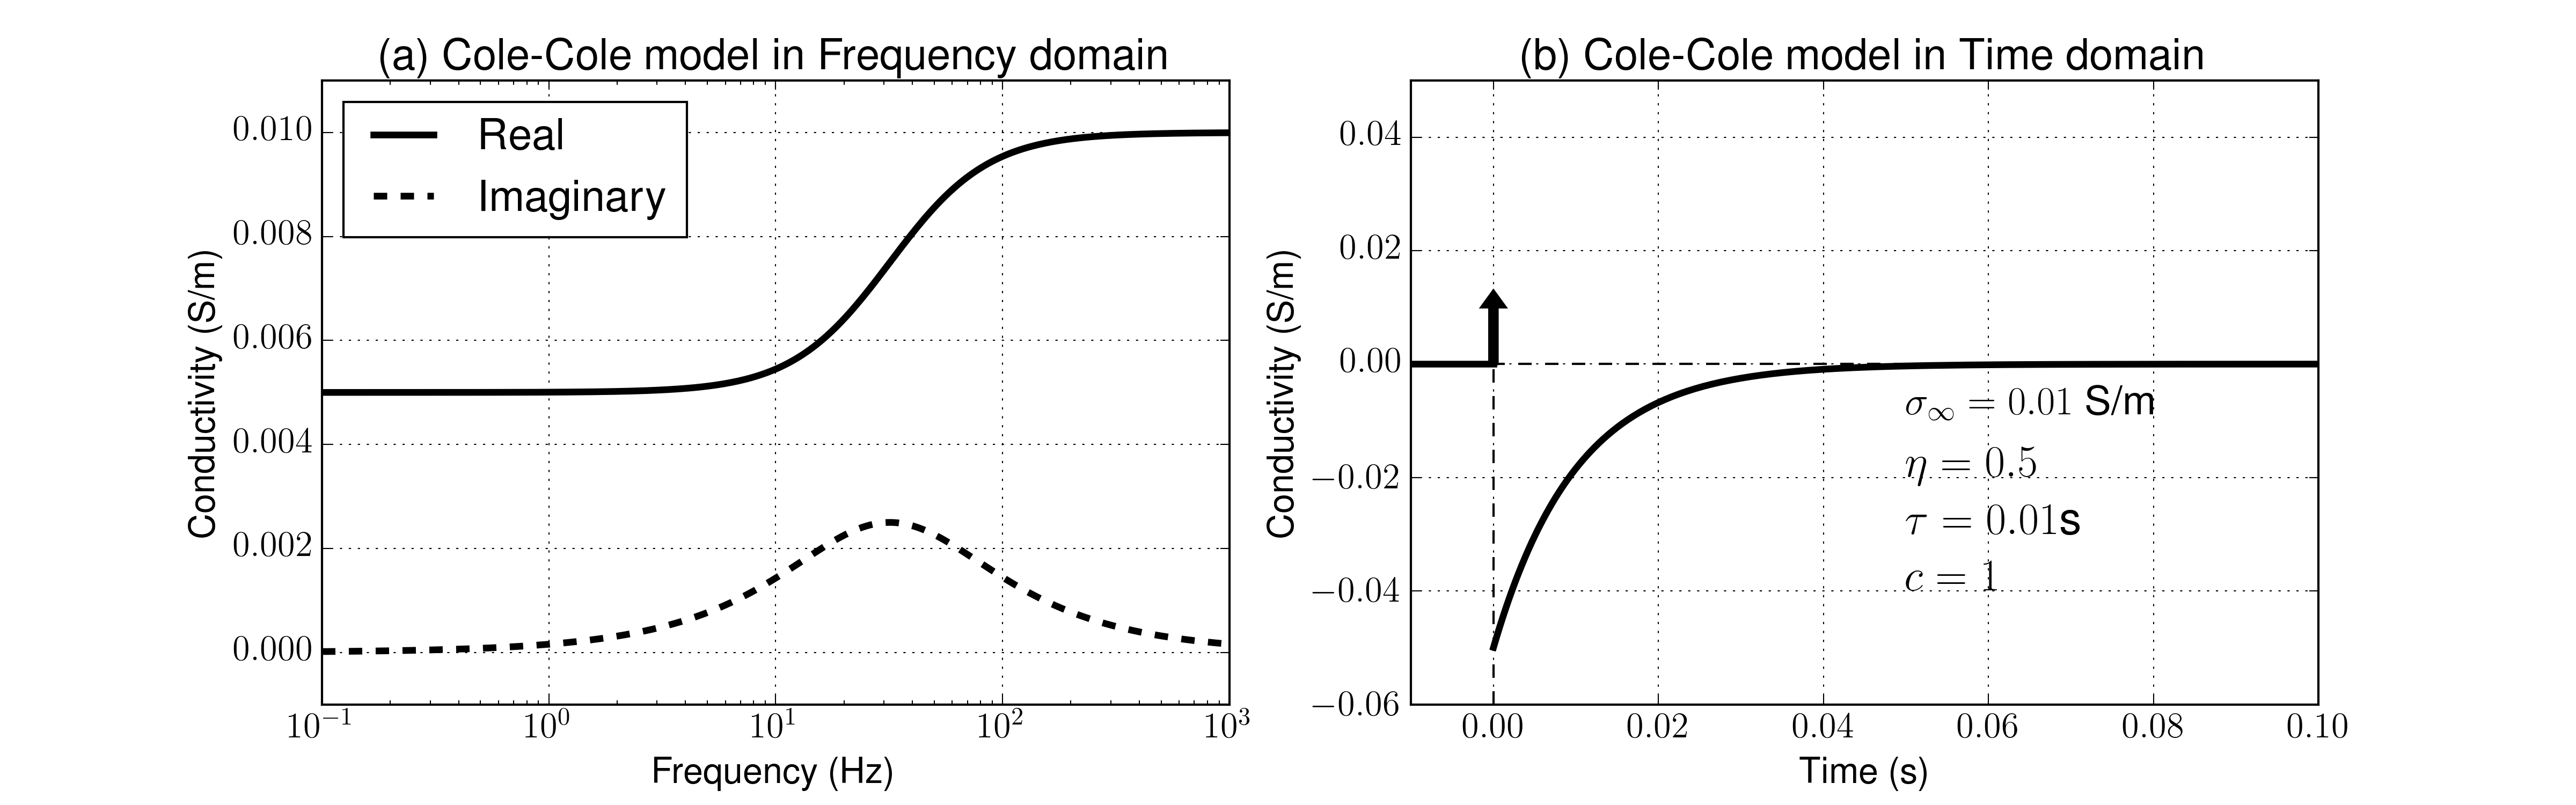
\includegraphics[width=1.0\textwidth]{figures/FDandTDCole.png}}
  \caption{Cole-Cole model in frequency domain (a) and time (b) domain. Used Cole-Cole parameters are $\siginf$ = $10^{-2}$ S/m, $\eta $ = 0.5, $\tau$ = 0.01, and $c$=1.}
  \label{Fig:FDandTDCole}
\end{figure}

%% =============================================================================
%% Section. Decomposition of observed responses
%% =============================================================================

\section{Decomposition of observed responses}
IP effects in the observed data are coupled with EM effects. We need to decompose these effects in the observation to isolate only data associated with the IP phenomena.  
Maxwell's equations in time domain with a quasi-static approximation are written as:
\begin{linenomath*}
\begin{equation}
  \curl{\e} = -\frac{\partial \b}{\partial t},
  \label{eq: total_farad}
\end{equation}
\end{linenomath*}
\begin{linenomath*}
\begin{equation}
  \curl{\frac{1}{\mu}\b} - \j= \j_{s},
  \label{eq: total_coulomb}
\end{equation}
\end{linenomath*}
where $\e$ is the electric field ($V/m$), $\b$ is the magnetic flux density ($Wb/m^2$) and $\mu$ is the magnetic permeability ($H/m$). Here $\j$ is the conduction current. In the frequency domain, this conduction current, $\J$ is related to conductivity via Ohm’s law: $\J(\omega) = \sigma(\omega)\E(\omega)$ where $\E$ is the electric field. 
Converting this relationship to time domain using the inverse Fourier transform yields:
\begin{linenomath*}
\begin{equation}
  \j(t) = \sigma(t)\otimes \e(t) = \int_0^t \sigma(u) e(t-u) du.
  \label{eq: ohms_law_convolution}
\end{equation}
\end{linenomath*}
where $\otimes$ indicates time convolution for a causal signal.  
Thus the current density depends upon the previous history of the electric field.
As in \cite{Smith1988a}, we let total fields as $\e = \e^{F} + \e^{IP}$, $\b = \b^{F} + \b^{IP}$ and $\j = \j^{F} + \j^{IP}$, where superscript $F$ indicates fundamental and $IP$ is induced polarization. 
Here fundamental fields indicate EM fields without IP effects. 
Substituting into equations (\ref{eq: total_farad}) and (\ref{eq: total_coulomb}) yields the following sequences:
\begin{linenomath*}
\begin{equation}
  \curl({\e^{F}+\e^{IP}}) = -\frac{\partial}{\partial t} (\b^{F}+\b^{IP}),
\end{equation}
\end{linenomath*}
\begin{linenomath*}
\begin{equation}
  \curl\frac{1}{\mu}(\b^{F}+\b^{IP}) - (\j^{F}+\j^{IP})= \j_{s}.
\end{equation}
\end{linenomath*}

The fundmental equations can be written as
\begin{linenomath*}
\begin{equation}
  \curl \e^{F} = -\frac{\partial \b^{F}}{\partial t},
  \label{eq: eq_primary_farad}
\end{equation}
\end{linenomath*}
\begin{linenomath*}
\begin{equation}
  \curl{\frac{1}{\mu}\b^{F}} -\j^{F} = \j_s.
  \label{eq: eq_primary_coulomb}
\end{equation}
\end{linenomath*}
Here
\begin{linenomath*}
\begin{equation}
  \j^{F} = \siginf\e^{F}.
  \label{eq: jF}
\end{equation}
\end{linenomath*}

Substituting the fundamental fields into equations (\ref{eq: total_farad}) and (\ref{eq: total_coulomb}) yields the expressions for the IP fields 
\begin{linenomath*}
\begin{equation}
  \curl \e^{IP} = -\frac{\partial \b^{IP}}{\partial t},
  \label{eq: eq_secondary_farad}
\end{equation}
\end{linenomath*}
\begin{linenomath*}
\begin{equation}
  \curl{\frac{1}{\mu}\b^{IP}} = \j^{IP}.
  \label{eq: eq_secondary_coulomb}
\end{equation}
\end{linenomath*}

Let $F[\cdot]$ denote operator associated with Maxwell’s equations, and let $d$ denote the observations that include both EM and IP effects. 
Keeping the same notation, we can obtain $d = d^{F} + \dip$, where $d^F$ and $\dip$ are fundamental and IP responses, respectively. 
Based on this, we define the IP datum as 
\begin{linenomath*}
\begin{equation}
  \dip = d - d^{F} = F[\sigma(t)]-F[\siginf].
    \label{eq: IPdatum_syn}
\end{equation}
\end{linenomath*}
Here $F[\siginf]$ corresponds to the fundamental response ($d^F$). 
This subtraction process acts as an EM decoupling process, which removes the EM effects from the measured responses. This is the same procedure that formed the basis of work by \cite{routh2001}. 

%% ============================================================
%% Section. Pseudo-chargeability for inductive sources
%% ============================================================
\section{Pseudo-chargeability for inductive sources}
%% later
% A major difference of the inductive source from the galvanic source is the absence of the steady-state electric field. 
% This generates a principal difference on the IP response for both inductive and galvanic sources. 
% To examine this, we define the IP current ($\j^{IP}$) as
Combining equations (\ref{eq: sigma_time}) and  (\ref{eq: ohms_law_convolution}) writing $j(t)=j^F + j^{IP}$ we obtain
\begin{linenomath*}
\begin{equation}
  \j^{IP} = \siginf \e^{IP} + \j^{pol},
  \label{eq:IP_current}
\end{equation}
\end{linenomath*}
where the polarization current ($\j^{pol}$) is
\begin{linenomath*}
\begin{equation}
  \j^{pol}(t) = \dsig(t)u(t) \otimes \e(t).
  \label{eq:polarization_current}
\end{equation}
\end{linenomath*}

If the electric field has different characteristics for the inductive and galvanic sources this will generate different features in the polarization current.  
We consider two cases: a) galvanic source without EM induction and b) inductive source with EM induction. The first case corresponds to EIP (\cite{seigel1959}), and the second is ISIP.
Figure \ref{F:DCEM_F_current} shows the amplitude of the fundamental electric field ($\e^{F}$) in the earth for those two cases. 
For the galvanic source, the electric field is instantaneous due to the steady-state electric field (Figure \ref{F:DCEM_F_current} (a)). 
However, for the inductive source, the electric field in the off-time is not zero, but increases to a peak and then decays as shown in Figure \ref{F:DCEM_F_current} (b). 
The polarization current for the two different sources will be significantly affected by these different electric fields. 
To capture this difference in a linearized kernel for the IP response, we define pseudo-chargeability ($\peta(t)$) as 
\begin{linenomath*}
\begin{equation}
  \peta(t) = -\frac{\j^{pol}(t)}{\j^{\ ref}},
  \label{eq:pseudochargeability_0}
\end{equation}
\end{linenomath*}
where the reference current ($\j^{ref}$) is defined as 
\begin{linenomath*}
\begin{equation}
  \j^{\ ref} = \siginf \eref.
  \label{eq:reference_current}
\end{equation}
\end{linenomath*}
Here $\eref$ is the reference electric field and both $\j^{\ ref}$ and $\eref$ are static fields that are independent of time. 
The pseudo-chargeability defined in equation (\ref{eq:pseudochargeability_0})  is the ratio of  the polarization current to the reference current. This is a small quantity and it plays an essential role in our linearization. 

To evaluate the pseudo-chargeability, we have to identify the reference current or reference electric fields. For the EIP case, the electric field, when there is no IP present, is independent of time as shown in Figure \ref{F:DCEM_F_current}(a) and any on-time value of the field can serve as a reference. For the inductive source however, the electric field does not achieve a steady-state, but increases to the peak then decreases. Our choice of the reference electric field is the maximum of the $\e^{F}$ and the  time at which the  maximum electric field occurs is our reference time ($t^{\ ref}$).
Each pixel in the Earth has its own reference electric field and time thus  both $\eref$ and $t^{\ ref}$ have a 3D distribution. 
For both EIP and ISIP cases, we mathematically present our choice of the reference electric field as
\begin{linenomath*}
\begin{equation}
  \eref = \e^{F}(t) \otimes \delta(t-t^{\ ref}). 
  \label{eq:reference_electricfield}
\end{equation}
\end{linenomath*}
The reference time for the EIP case can be any time in the on-time, because the fundamental electric field for the EIP case does not change in on-time. 

By rearranging equation (\ref{eq:pseudochargeability_0}), we obtain 
\begin{linenomath*}
\begin{equation}
  \j^{pol} = -\jref\peta(t). 
  \label{eq:polarization_current_concept}
\end{equation}
\end{linenomath*}
This states that the polarization current has an opposite direction to the reference current, and is proportional to the pseudo-chargeability ($\peta(t)$). 
This conceptual model about the polarization current shown in equation (\ref{eq:polarization_current_concept}) is consistent with \cite{seigel1959}'s result. We note, that for any pixel, even though  $\eref$  attains the same value for an ISIP survey as for an EIP survey, the pseudo-chargeability resulting from  an ISIP survey  will be less than that from an EIP survey. We can infer from this that  linearization techniques, which  have worked so well in EIP problems, should be successful in ISIP problems. 

\begin{figure}  
  \figbox*{}{}{
  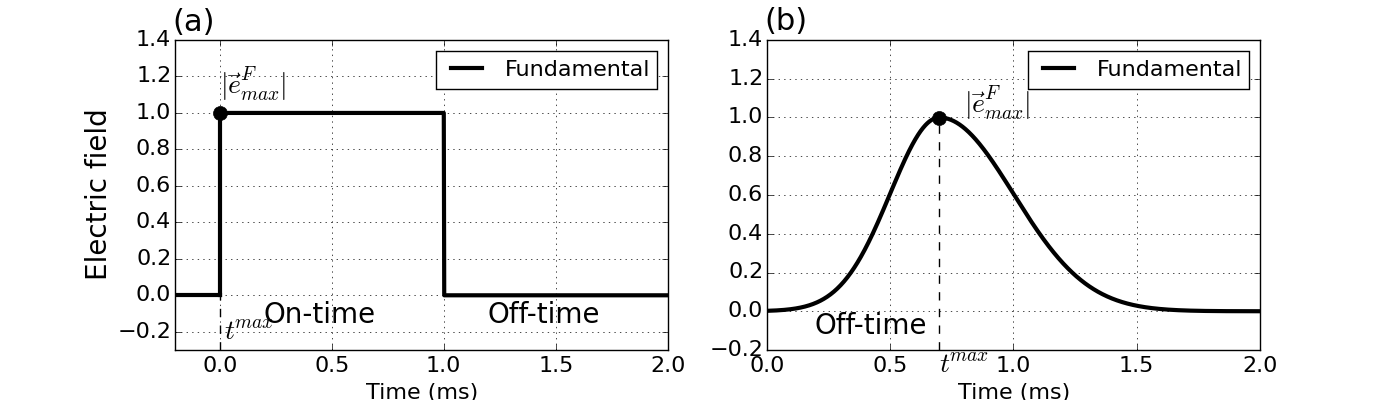
\includegraphics[width=1.0\textwidth]{figures/DCEM_F_current.png} }
  \caption{Conceptual diagram for the amplitude of the fundamental electric fields. (a) EIP and (b) ISIP cases.}
  \label{F:DCEM_F_current}
\end{figure}   

%% ============================================================
%% Section. Linearization
%% ============================================================
\section{Linearization}
Following from the methodologies in EIP, our goal is to express the IP response ($\dip$) as a function of the pseudo-chargeability $(\peta(t))$ in time  $\dip(t) = J[\peta(t)]$, where $J[\cdot]$ is a linear operator which is independent of time. In doing this we first consider a general EM system which is applicable to galvanic or inductive sources. 
For any pixel  volume in the earth the amplitude and direction of the  electric field can vary dramatically  in time and this results in a complicated  IP charging process. If substantial polarization currents are developed however, they will correspond to a maximum electric field or reference current aligned in a constant direction. Our formulation focuses on this aspect. We assume that the final large scale IP response observed in the data is the result of  pixels being charged with an electric field in a specific direction but with a variable amplitude. Let $\e(t)$ be approximated as
\begin{linenomath*}
\begin{equation}
  \e(t) \approx \eref w^e(t),
  \label{eq: e_with_eref}
\end{equation}
\end{linenomath*}
where $w^e(t)$ is defined as:
\begin{linenomath*}
\begin{equation}
  w^e(t) = P_0[w^{ref}(t)],
  \label{eq: we}
\end{equation}
\end{linenomath*}
where a projection ($P_0[\cdot]$) of an arbitrary function, $f(t)$ is
\begin{linenomath*}
\begin{equation}
  P_0[f(t)] = \left\{ 
  \begin{array}{l l}
    f(t) & f(t) \ge 0 \\
    0 & \text{if } f(t) < 0, 
  \end{array}\right.
  \label{eq: P0}
\end{equation}
\end{linenomath*}
and
\begin{linenomath*}
\begin{equation}
  w^{ref}(t) = \frac{\e^F(t)\cdot\eref}{\eref\cdot\eref}.
  \label{eq: wref}
\end{equation}
\end{linenomath*}
Here $w^{ref}(t)$ is a dimensionless function that prescribes the time history of the electric field at each location along the direction of the chosen reference electric field ($\eref$).  Negative values of  $w^{ref}(t)$ are set to zero in accordance with our conceptual model that polarization currents have an opposite direction to the reference current (equation (\ref{eq:polarization_current_concept})).
We redefine the pseudo-chargeability as
\begin{linenomath*}
\begin{equation}
    \peta(t) = \peta^{I}(t)\otimes w^e(t).
    \label{eq: pseudochargeability}
\end{equation}
\end{linenomath*}
Polarization current, $\j^{pol}$ can be approximated with equation (\ref{eq: intrinsic_peta}) as
\begin{linenomath*}
\begin{equation}
  \j^{pol}(t) \approx - \peta^{I}(t)\otimes w^e(t)\jref.
\end{equation}
\end{linenomath*}
Substituting this into equation (\ref{eq:IP_current}) yields
\begin{linenomath*}
\begin{equation}
  \j^{IP}(t) \approx \siginf\e^{IP}(t) - \peta^{I}(t)\otimes w^e(t)\jref
\end{equation}
\end{linenomath*}
and this yields
\begin{linenomath*}
\begin{equation}
  \j^{IP}(t) \approx \siginf\e^{IP}(t) -\jref\peta(t).
  \label{eq: jip_EMIP}
\end{equation}
\end{linenomath*}

The first term, $\siginf e^{IP}(t)$ is usually omitted (\cite{Smith1988a}). Here we include it and explore the conditions in which it is important. 
Because the reference current is static, any time-dependency in the polarization currents is encapsulated in the pseudo-chargeability. The buildup and decrease of polarization currents is a slow process and we assume therefore that this process does not produce induction effects ($\frac{\partial \b^{IP}}{\partial t} \approx 0$) and therefore we can write 
\begin{linenomath*}
\begin{equation}
  \e^{IP} \approx  \e^{IP}_{approx} = -\grad\phi^{IP}.
  \label{eq: eip_approx}
\end{equation}
\end{linenomath*}

By taking the divergence of  equation (\ref{eq: jip_EMIP}), substituting  $\e^{IP}$ with equation (\ref{eq: eip_approx}), and carrying out some linear algebra, we obtain
\begin{linenomath*}
\begin{equation}
  \phi^{IP}(t) \approx -[\div \siginf\grad]^{-1}\div\jref\peta(t).
  \label{eq: phiIPapprox_general}
\end{equation}
\end{linenomath*}
By applying the gradient we obtain 
\begin{linenomath*}
\begin{equation}
    \e^{IP}_{approx} = \grad[\div \siginf\grad]^{-1}\div\jref\peta(t).
    \label{eq: eip_approx_full}
\end{equation}
\end{linenomath*}
Thus, the electric field due to the IP effect can be expressed as a function of $\peta(t)$ in time. 
This form is also applicable to the  EIP case.   

For an inductive source, the data is often either $\b$ or its time derivative and hence we also need to compute $\b^{IP}$ or its time derivative.
For this, we first compute $\j^{IP}$ then use Biot-Savart law to compute $\b^{IP}$ or $\frac{\partial \b^{IP}}{\partial t}$. 
Substituting equation (\ref{eq: eip_approx_full}) into equation (\ref{eq: jip_EMIP}), the approximated IP current density, $\j^{IP}_{approx}$ can be expressed as
\begin{linenomath*}
\begin{equation}
  \j^{IP}(t) \approx \j^{IP}_{approx} = \bar{S}\jref\peta(t),
  \label{eq: jip_approx}
\end{equation}
\end{linenomath*}
where
\begin{linenomath*}
\begin{equation}
  \bar{S} = \siginf\grad[\div \siginf\grad]^{-1}\div-\bar{I}
\end{equation}
\end{linenomath*}
and $\bar{I}$ is an identity tensor. 
Applying Biot-Savart law we have:
\begin{linenomath*}
\begin{equation}
  \b^{IP}_{approx}(\vec{r}; t) = \frac{\mu_0}{4\pi}\int_{\Omega}  \frac{\bar{S}\j^{\ ref}(\vec{r}_s)\times\hat{r}}{|\vec{r}-\vec{r}_s|^2}\peta(t)d\vec{r}_s.
  \label{eq: BiotbIP_approx}
\end{equation}
\end{linenomath*}
If $\siginf\e^{IP}$ is omitted in  $\j^{IP}$ then the tensor, $\bar{S}$ becomes $-\bar{I}$. 
In this situation, the IP current is same as the polarization current, and always has opposite direction to the reference current. 
This reversed current with Biot-Savart law provides physical understanding of the negative transients in ATEM data when the earth include a chargeable body. 

Observed data are often time derivative of $\b$, hence by taking time derivative to the equation (\ref{eq: BiotbIP_approx}), we obtain
\begin{linenomath*}
\begin{equation}
  -\frac{\partial\b^{IP}_{approx}}{\partial t}(\vec{r}; t) = \frac{\mu_0}{4\pi} \int_{\Omega}  \frac{\bar{S}\jref(\vec{r}_s)\times\hat{r}}{|\vec{r}-\vec{r}_s|^2} \Big( -\frac{\partial \peta(t)}{\partial t} \Big) d\vec{r}_s.
  \label{eq: BiotbIPdt_approx}
\end{equation}
\end{linenomath*}
Here we have chosen to keep the minus signs in equation (\ref{eq: BiotbIPdt_approx}) so that the sign of input of the kernel, $-\frac{\partial \peta(t)}{\partial t}$ is positive when $\peta(t)$ is decaying in time. 
Accordingly, the IP datum is given by  $-\frac{\partial\b^{IP}}{\partial t}$. 

The IP fields shown in equations (\ref{eq: eip_approx_full}), (\ref{eq: BiotbIP_approx}) and (\ref{eq: BiotbIPdt_approx}) are linear functionals of $\peta(t)$ and  the equations can be discretized in space as
\begin{linenomath*}
\begin{equation}
  \mathbf{d}^{IP}_i = \mathbf{J}\peta_i,
  \label{eq: dIP_lineareq}
\end{equation}
\end{linenomath*}
where $\mathbf{J}$ is corresponding sensitivity matrix and the subscript $i$ indicates $i^{th}$ time channel. 
In particular when the observed datum is the time derivative of $\b$, the linear relationship can be written as 
\begin{linenomath*}
\begin{equation}
  \mathbf{d}^{IP}_i = \mathbf{J}(-\frac{\partial \peta}{\partial t}\Big|_i).
  \label{eq: dIP_lineareq_dbdt}
\end{equation}
\end{linenomath*}
A detailed description for the discretization of the linearized kernel is shown in sections \ref{section:maxwell_discrete} and \ref{section:linearkernel_discrete}. 
The representation in equation (\ref{eq: dIP_lineareq}) is valid for galvanic and inductive sources but the two assumptions: a) $\e \approx \eref w^e(t)$ and b) $\e^{IP} \approx -\grad\phi^{IP}$ need to be tested numerically for the case of inductive sources. 

%% =============================================================================
%% Section. IP inversion methodology
%% =============================================================================

\section{IP inversion methodology}

%%% ===========================================================================
%%% SUBSECTION
\subsection{3D IP inversion with a linearized kernel}
The linear inverse problem to recover chargeability is straightforward and is described in \cite{doug1994}. 
We rewrite equation (\ref{eq: dIP_lineareq}) as
\begin{linenomath*}
\begin{equation}
  \mathbf{d}^{pred} = \mathbf{J}\mathbf{m},
  \label{eq9}
\end{equation}
\end{linenomath*}
where $\mathbf{J}$ is the  sensitivity matrix of linear problem, which corresponds to $\mathbf{J}$ shown in equation (\ref{eq: dIP_lineareq}) 
Here, $\mathbf{d}^{pred}$ is IP responses at $i^{th}$ time channel ($\mathbf{d}^{IP}_i$), $\mathbf{m}$ is distributed model parameters, which can be either $\peta_{i}$ or $-\frac{\partial \peta}{\partial t}\big|_i$. 
In our work here we invert each time channel of $d^{IP}$, separately. 

The solution to the inverse problem is the model $\mathbf{m}$ that solves the optimization problem
\begin{linenomath*}
\begin{equation}
  minimize \ \phi =  \phi_d(\mathbf{m}) + \beta\phi_m(\mathbf{m})\nonumber \\
  s.t. \ 0 \le \mathbf{m},
  \label{eq10}
\end{equation}
\end{linenomath*}
where $\phi_d$ is a measure of data misfit, $\phi_m$ is a user-defined model objective function and $\beta$ is regularization or trade-off parameter. We solve this optimization problem using a projected Gauss-Newton method (\cite{Kelley}). 
The value of $\beta$ in the iteration of this non-linear inversion is determined using a cooling technique where $\beta$ is progressively reduced from some high value. The inversion is stopped when the tolerance is reached (cf. \cite{DougTutorial, Kang2014}). 

We use the sum of the squares to measure data misfit
\begin{linenomath*}
\begin{equation}
  \phi_d = \| \mathbf{W_d}(\mathbf{A}\mathbf{m}-d^{obs}|)\|^2_2 =
  \sum^N_{j=1}(\frac{\mathbf{d}^{pred}_j-\mathbf{d}^{obs}_j}{\epsilon_j}),
  \label{eq11}
\end{equation}
\end{linenomath*}
where $N$ is the number of the observed data and $\mathbf{W_d}$ is a diagonal data weighting matrix which contains the reciprocal of the estimated uncertainty of each datum ($\epsilon_j$) on the main diagonal,  $\mathbf{d}^{obs}$ is a vector containing the observed data, $\mathbf{d}^{pred}$ is a vector containing calculated data from a linear equation given in equation (\ref{eq9}).
The model objective function, $\phi_m$ is a measure of amount structure in the model and upon minimization this will generate a smooth model which is close to a reference model, $m_{ref}$. 
We define $\phi_m$ as
\begin{linenomath*}
\begin{equation}
  \phi_m = \alpha_s\| \mathbf{W}_s\mathbf{W}(\mathbf{m}-\mathbf{m}_{ref})\|^2_2+
       \alpha_x\| \mathbf{W}_x\mathbf{W}(\mathbf{m}-\mathbf{m}_{ref})\|^2_2+ \nonumber \\
       \alpha_y\| \mathbf{W}_y\mathbf{W}(\mathbf{m}-\mathbf{m}_{ref})\|^2_2+
       \alpha_z\| \mathbf{W}_z\mathbf{W}(\mathbf{m}-\mathbf{m}_{ref})\|^2_2,
  \label{eq12}
\end{equation}
\end{linenomath*}
where $\mathbf{W}_s$ is a diagonal matrix, and $\mathbf{W}_x$, $\mathbf{W}_y$ and $\mathbf{W}_z$ are discrete approximations of the first derivative operator in $x$, $y$ and $z$ directions, respectively.  
The $\alpha$'s are weighting parameters that balance the relative importance of producing small or smooth models.

We are inverting each time channel of $\dip$ datum, separately. Thus, we do not have intrinsic depth resolution. This could be overcome if there were multiple receivers for each transmitter. To compensate for this, and similar to the magnetic inversion (\cite{LiMag3D}), we apply depth weighting through model weighting matrix ($\mathbf{W}$):
\begin{linenomath*}
\begin{equation}
    \mathbf{W} = \mathbf{diag}(\mathbf{z-z_0})^{1.5},
    \label{eq: weight_mat}
\end{equation}
\end{linenomath*}
where $\mathbf{z}$ and $\mathbf{z_0}$ are discretized depth locations and reference depth in 3D domain.

%% ===========================================================================
%% SUBSECTION
\subsection{Extracting intrinsic IP parameters}
\label{section: extract_intrinsicIP}
The output of our IP inversion is a 3D distribution of the pseudo-chargeability at multiple time channels. 
As its name suggests, pseudo-chargeability is not an intrinsic IP parameter like chargeability, but it is convoluted property between $\peta^{I}(t)$ and $w^{e}(t)$:
\begin{linenomath*}
\begin{equation}
  \peta(t) = \peta^{I}(t)u(t) \otimes w^e(t),
  \label{eq: pseudochargeability_petaI}
\end{equation}
\end{linenomath*}
with the definition of intrinsic pseudo-chargeability (equation (\ref{eq: intrinsic_peta})).
We would now like to use the $\peta(t)$ as the “data” and recover intrinsic parameters such as $\eta, \tau, c$ in a Cole-Cole model. Assuming a Debye model ($c$=1), we obtain
\begin{linenomath*}
\begin{equation}
    \peta^{I}(t) = \frac{\eta}{(1-\eta)\tau}e^{-\frac{t}{(1-\eta)\tau}},
    \label{eq: intrinsic_peta_debye}
\end{equation}
\end{linenomath*}
Since we have $\siginf$ we can compute $w^e(t)$, which is time history of the electric field. 
Accordingly, we can unravel the recovered pseudo-chargeability to extract intrinsic IP parameters such as chargeability($\eta$) and time constant ($\tau$). 
We use a gradient-based optimization, we need the sensitivity function for the pseudo-chargeability (equation (\ref{eq: pseudochargeability_petaI})) with regard to $\eta$ and $\tau$. 
To simplify this procedure, we rewrite intrinsic pseudo-chargeability as 
\begin{linenomath*}
\begin{equation}
  \peta^{I}(t) = a e^{-bt},
\end{equation}
\end{linenomath*}
where $a = \frac{\eta}{(1-\eta)\tau}$ and $b = \frac{t}{(1-\eta)\tau}$. 
Then we take derivative of $\peta(t)$ with regard to $a$ and $b$:
\begin{linenomath*}
\begin{equation}
  \frac{\partial \peta(t)}{\partial a} = e^{-bt} \otimes w^e(t),
\end{equation}
\end{linenomath*}
\begin{linenomath*}
\begin{equation}
  \frac{\partial \peta(t)}{\partial b} = -ate^{-bt} \otimes w^e(t).
\end{equation}
\end{linenomath*}
With these sensitivity functions, we can set up an inverse problem, and recover $a$ and $b$. 
Chargeability and time constant can be obtained by using $a$ and $b$:
\begin{linenomath*}
\begin{equation}
  \eta =  \frac{1}{(1-a/b)b},
\end{equation}
\end{linenomath*}
\begin{linenomath*}
\begin{equation}
  \tau =  \frac{a}{b}.
\end{equation}
\end{linenomath*}
We apply this inversion separately to each cell in the recovered pseudo-chargeability  in a manner similar to \cite[]{Yuval1997}.
For the better representation of time-dependent conductivity, a different parameterization such as stretched-exponential (\cite{Kohlrausch1854}) or Cole-Cole model with variable $c$ can be implemented. 

% %%% ===========================================================================
% %%% SUBSECTION
\subsection{Handling multiple transmitters in ATEM surveys}
\label{subsection: Handling multiple transmitters in ATEM surveys}
The work for inductive sources in the previous sections has been developed for a single transmitter and  3D information about chargeability can be obtained if there are multiple receivers. For ATEM data however, we have only a single receiver location for each transmitter but we have multiple transmitter locations. 
Our goal is to alter the problem to work with an effective pseudo-chargeability. 

Considering this situation where the survey includes multiple transmitters, we define IP datum for $k$-th transmitter as 
\begin{linenomath*}
\begin{equation}
  \dip_k(t) = \sum_{i=1}^{nC}J_{k,i}\peta^k_i (t), \ \ k=1, \ldots, nTx,
  \label{eq: dip_kthTx}
\end{equation}
\end{linenomath*}
where $nTx$ is the number of transmitters, $nC$ is the number of cells in the domain, and $J_{k,i}$ indicates an element of the Jacobian matrix for an $k$-th transmitter and $i$-th cell. We want to write this as 
\begin{linenomath*}
\begin{equation}
  \dip_k(t) = \sum_{i=1}^{nC}J_{k,i}\peta_i (t), \ \ k=1, \ldots, nTx,
  \label{eq: dipeff_kthTx}
\end{equation}
\end{linenomath*}
Here $\peta(t)$ stands for an effective pseudo-chargeability.
The waveforms are different for different transmitters and hence this cannot be exact. To examine the implications we look at the contribution of an $i$-th pixel to the $nTx$ data set at a single time. 
It is 
\begin{linenomath*}
\begin{equation}
  \hat{d}^{IP}_i(t) =\sum_{k=1}^{nTx} J_{k,i} \peta^k_i(t), \ \ i=1, \ldots, nC.
  \label{eq: dip_hat}
\end{equation}
\end{linenomath*}
% Accordingly, the sum of the IP data can be expressed as $\Sigma_{k=1}^{nTx}\dip_k(t) = \Sigma_{i=1}^{nC}\hat{d}^{IP}_i(t)$.
Here our goal is to replace $\peta_k$ with a scalar $\peta$ and make the contribution the same. That is 
\begin{linenomath*}
\begin{equation}
  \tilde{d}^{IP}_i(t) =\sum_{k=1}^{nTx} J_{k,i} \peta_i(t), \ \ i=1, \ldots, nC.
  \label{eq: dip_tilde}
\end{equation}
\end{linenomath*}
The effective pseudo-chargeability at $i$-th pixel that minimizes the squared difference between these quantities is 
\begin{linenomath*}
\begin{equation}
  \peta_i(t) = \frac {\Sigma_{k=1}^{nTx} J_{k,i}\peta^k_i(t)} {\Sigma_{k=1}^{nTx} J_{k,i}}, \ \ i=1, \ldots, nC.
  \label{eq: petaeff}
\end{equation}
\end{linenomath*}
Similar to the projection applied $w^{\ ref}(t)$ (equation (\ref{eq: we})) to preserve the polarization current aligned in the opposite direction of the reference current, we projects any negative values in effective pseudo-chargeability to zero. 
Considering this projection, we redefine the effective pseudo-chargeability as 
\begin{linenomath*}
\begin{equation}
  \peta_i(t) = P_0\Big[\frac {\Sigma_{k=1}^{nTx} J_{k,i}\peta^k_i(t)} {\Sigma_{k=1}^{nTx} J_{k,i}}\Big], \ \ i=1, \ldots, nC.
  \label{eq: petaeff_pos}
\end{equation}
\end{linenomath*}
With the above understanding about how $\peta$ relates to the $\peta^k$ from each transmitter we can proceed as usual (equation (\ref{eq: dIP_lineareq})). 
In additon, by letting 
\begin{linenomath*}
\begin{equation}
  \peta_i(t) = \peta^I(t)u(t) \otimes w^e_i(t),
\end{equation}
\end{linenomath*}
we define effective $w^e_i(t)$ as 
\begin{linenomath*}
\begin{equation}
  w^e_i(t)= P_0\Big[\sum_{k=1}^{nTx} a^k_i w^{e \ k}_i(t)\Big], \ \ i=1, \ldots, nC,
  \label{eq: we_eff}
\end{equation}
\end{linenomath*}
where normalized weight ($a^k_i$) is 
\begin{linenomath*}
\begin{equation}
  a^k_i = \frac {J_{k,i}} {\Sigma_{k=1}^{nTx} J_{k,i}}, \ \ i=1, \ldots, nC.
  \label{eq: normalized_weights}
\end{equation}
\end{linenomath*}
% Doug
% This includes all grounded surveys with multiple transmitters and to a single source inductive EIP surveys.

%%% ===========================================================================
%%% SUBSECTION
\subsection{IP inversion procedure}
As seen in the previous sections the extraction of IP information from TEM data has multiple steps. These include: (1) invert TEM data and recover a 3D conductivity model ($\sigma_{est}$). 
(2) Forward modelling $\sigma_{est}$ to obtain the fundamental response $d^F$ and subtracting it from the observations to obtain $\dip$ data.
(3) Invert  $\dip$ data to recover pseudo-chargeability model at individual time channels using the relationship in equation (\ref{eq: dIP_lineareq}). 
(4) Further process the inversion outputs at multiple time-channels  to estimate the Cole-Cole, or equivalent IP parameters.

In the following we investigate each of the above steps via numerical simulations and test the validity of our assumptions. 

%% =============================================================================
%% Section. Numerical experiments
%% =============================================================================

\section{Numerical experiments}
\label{section: numerical_examples}
For our numerical experiments we concentrate upon coincident loop ATEM surveys. This choice is made because of the observed negative transients that are direct indicators of IP phenomena (\cite{Kratzer2012,Kang2015a,Kang2015b,Doug2015}), and the extensive  use of this survey  by industry.  

We begin with a simple IP model composed of  a chargeable block in a half-space as shown in Figure~\ref{F: IPModel}.
Cole-Cole parameters of block are  $\eta=$0.2, $\tau=$0.005 and $c=$1.
The conductivity  of the half-space, ($\sigma_1$) is  $10^{-3}$ S/m, whereas $\sigma_2$, 
the conductivity at infinite frequency ($\siginf$) for the chargeable body, is variable.  
We consider three cases: a) canonical ($\sigma_2=\sigma_1$), b) conductive ($\sigma_2=10^2\times\sigma_1$) and c) resistive models ($\sigma_2=10^{-2}\times\sigma_1$).
The 3D earth is discretized with  $50\times50\times50$ m core cells and the number of cells in the domain is $41\times41\times40$.
The size of the chargeable body is $250\times250\times200$ m and the top boundary is located  $50$ m below the surface.
EMTDIP code (\cite{Marchant2014}) is used to compute forward ATEM responses that include IP effects. The survey consisting of 11 soundings along each of 11 lines is shown in Figure \ref{F: IPModel}a.
Data are from a  coincident-loop system and both Tx and Rx located 30 m above the surface; the radius of the loop is 10 m.
A step-off transmitter waveform is used and the range of the observed time channels is 0.01-60 ms. The observed responses can be either vertical component of $\b$ or $\frac{\partial \b}{\partial t}$.

In this section, we first decompose the observed responses and the total currents into fundamental and IP portions to aid in the basic understanding of IP effects in ATEM data. 
Second, we validate the linearized functional by computing the approximate IP current and IP responses, and comparing these  with the true values. 
Third, we investigate the feasibility of an effective pseudo-chargeability in 3D IP inversion. 
Fourth, we invert the IP data and recover 3D distributions of pseudo-chargeability at multiple times.  Lastly, we use the recovered pseudo-chargeabilities to examine the potential to extract intrinsic Cole-Cole parameters. 

\begin{figure}
  \figbox*{}{}{
  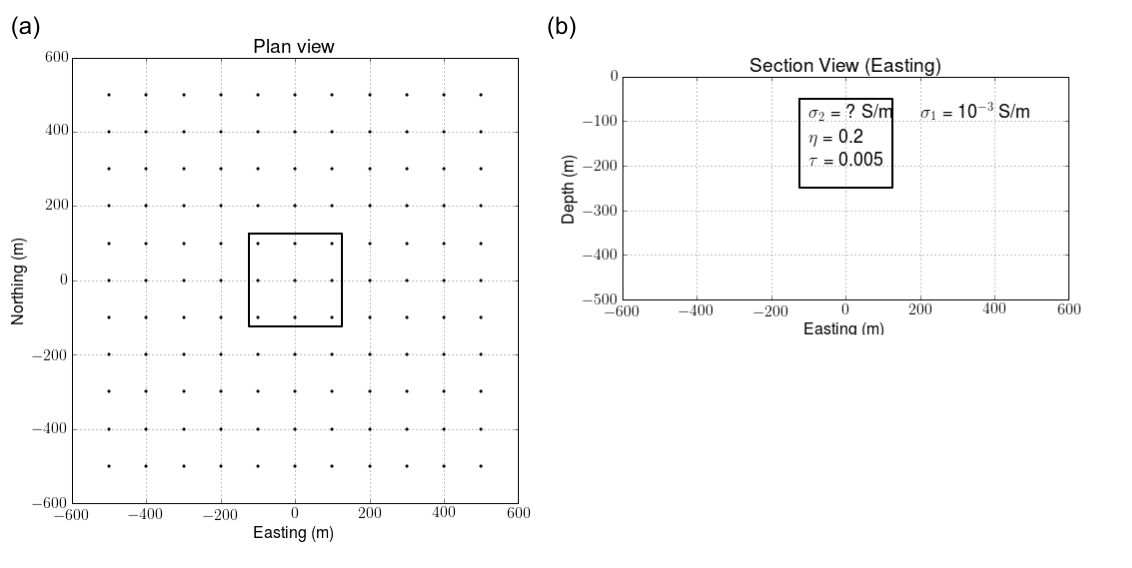
\includegraphics[width=1.0\textwidth]{figures/IPModel.png} }
  \caption{Plan (a) and section b) views of the IP model. Dashed line in (a) contours the boundary of the IP body. Solid circles in (a) denotes the sounding locations.}
  \label{F: IPModel}
\end{figure}
\clearpage

%%% ===========================================================================
%%% SUBSECTION
\subsection{IP responses}
Using the  EMTDIP code and carrying out two simulations, we compute the IP data via subtraction in equation (\ref{eq: IPdatum_syn}).
Figure \ref{F:Three_IPresp} shows the observed, fundamental, and IP responses at a sounding location above the center of the chargeable body for (a) canonical, (b) conductive and (c) resistive models. Both $b_z$ and $-\frac{\partial b_z}{\partial t}$ data are shown. 
The IP effects are most noticeable for the conductive body and we turn attention to this example first. The IP response starts to significantly affect the observations near 0.6 ms and the observed responses show a sign reversal near 1 ms. Beyond that time the signal is completely dominated by the IP. The dashed line in Figure \ref{F:Three_IPresp}b shows that after turn-off of the transmitter current, the IP current increases (as inferred by the magnitude of the $b_z$ field) until about 1 ms and then decreases. We interpret this in terms of charging and discharging phases and a vertical dashed line in the figure defines the two phases. In the charging phase at early times the EM effects dominate and IP signals are not expected to be observed. In the discharging phase, which occurs at  later time, the IP effects may eventually dominate the EM effects. The maximum of the $b_z^{IP}$ corresponds to the zero crossing for $\frac{\partial b_z^{IP}}{\partial t}$ but the times at which the IP signal becomes dominant are delayed compared to $b_z^{IP}$. By comparing the observations with the fundamental fields we see that the IP signal could be recognized in the $b_z$ data near 0.7 ms and near 2.0 ms in the $\frac{\partial b_z}{\partial t}$ data.

The plots for the canonical and resistive bodies show that the time that separates charging and discharging occurs earlier than for the conductive body. This is a reflection that the fundamental currents reside for a longer time in a conductor. For the canonical body, significant difference between the measured responses and the fundamental fields occur about 0.9 ms for $b_z$ and about 2 ms for $\frac{\partial b_z}{\partial t}$. The amplitudes of the IP responses are significantly smaller than those for the conductor.  Lastly, there is little IP signal for the resistive body; the IP signal much smaller than the fundmental response in given time range. This is a consequence of the small fundamental currents in the resistor. 

The decay curves from a sounding location  provides insight about the IP response but more is gleaned by looking at data from all  sounding locations in the ATEM survey. We focus on $b_z^{IP}$ for the conductive block at selected time channels. Figure \ref{F:IPresp_Plan} shows interpolated maps of the observed, fundamental and IP responses at (a) 0.86 ms and (b) 6.7 ms which are respectively included in the charging and discharging times. 
At 0.86 ms, the observations are dominated by the fundamental response and no negative values,  which are the signature of the IP effect, are observed. Subtracting the fundamental however, yields a residual $\dip$ data map that has a strong negative. This  example  shows that our EM decoupling procedure has worked satisfactorily.  At 6.7 ms, obtaining good IP data are easier identified because the observed data already show negative values. There is still a weak fundamental field and the subtraction process improves the $\dip$ response. The $\dip$ data at  0.86 ms and 6.7 ms shown in Figure \ref{F:IPresp_Plan} are of sufficient quality to be inverted. The decoupling has been carried out using the known background conductivity $\siginf$ which, in reality must be estimated. We address this issue later. 

\begin{figure}
  \figbox*{}{}{
  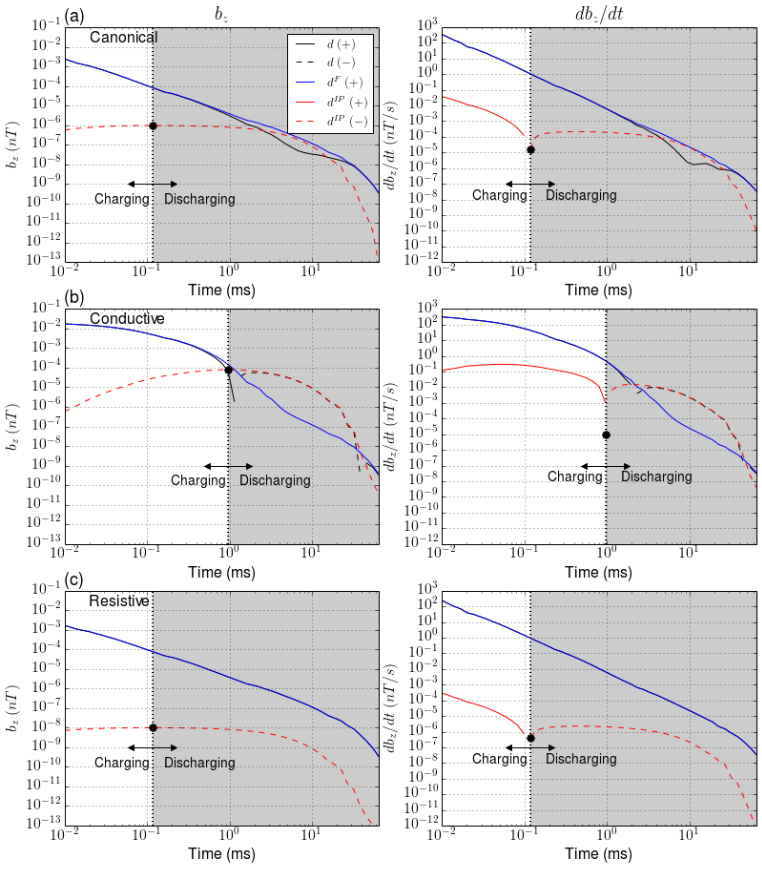
\includegraphics[width=1.\textwidth]{figures/Three_IPresp.png} }
  \caption{Time decaying curves of observation ($d$; black line), fundamental ($d^F$; blue line) and IP ($\dip$; red line) responses. All three cases: (a) canonical, (b) conductive and (c) resistive are presented. Right and left panels show $b_z$ and $\frac{\partial b_z}{\partial t}$. Black dotted line indicates the maximum polarization time.}
  \label{F:Three_IPresp}
\end{figure}
\begin{figure}
  \figbox*{}{}{
  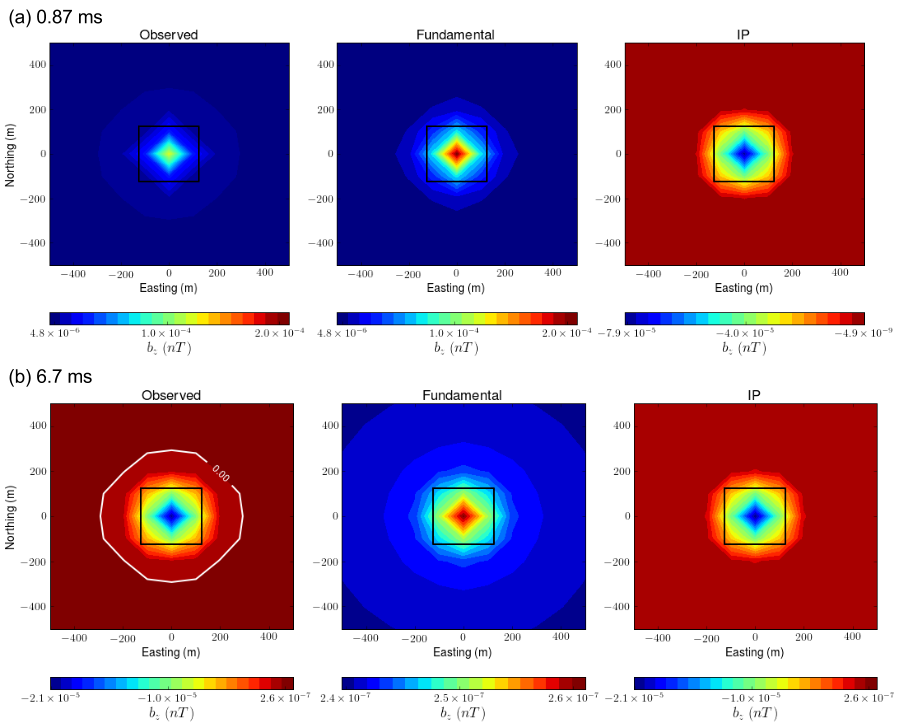
\includegraphics[width=1.\textwidth]{figures/IPresp_Plan.png} }
  \caption{Interpolated maps of observed (left panel), fundamental (middle panel) and IP (right panel) responses. Two time channels at (a) 0.86 ms and (b) 6.7 ms are presented. White line contours zero-crossing line in the observed response.  
  }
  \label{F:IPresp_Plan}
\end{figure}
\clearpage

%%% ===========================================================================
%%% SUBSECTION
\subsection{Polarization currents}
%Need some intro. 
To evaluate the polarization current shown in equation (\ref{eq:polarization_current}) for the linear functional, we assumed $\e(t) \approx \eref w^e(t)$ yielding $\j^{pol}(t) \approx -\j^{\ ref} \peta(t)$. This approximation will work when polarization currents developed from charging or discharging process correspond to a reference current alinged in constant direction. Accordingly, the choice of a reference electric field is crucial. The maximum electric field was chosen as the the reference electric field, which includes the time history of the fundamental electric field (equation (\ref{eq:reference_electricfield})). Since our focus here is the polarization current, analyzing the reference current is more insightful than the reference electric field. 

We first analyze the reference currents for canonical and conductive models shown in Figure ~\ref{F:ReferenceCurrent}a and b, respectively. 
Here a transmitter is located at (-200 m, 0 m, 30 m) and marked as white solid circle, where ($\cdot, \cdot, \cdot$) means a point at (easting, northing, depth).  
The fundamental current for the canonical model is circular, centered to the transmitter location, and is decaying as further away from this location. This feature is clearly captured in the referecne current as shown in Figure ~\ref{F:ReferenceCurrent}a. 
In the chargeable body, most of the currents is alinged in northing direction. 
Different from canonical case, when the earth contain a conductor, vortex current will be induced from the conductor, whereas the similar circular current centered to transmitter location still exists.  
Figure ~\ref{F:ReferenceCurrent}b shows that the reference current, which effectively incorporate both induced currents from the half-space earth and the embedded conductor.  
Especially in the body, the reference current is composed of linear currents alinged in northing direction and rotating currents in clockwise and counter-clockwise at plan and section view maps, respectively. 

Figures ~\ref{F:Polarizationcurrent_early} and ~\ref{F:Polarizationcurrent_late} show the plan and section view maps of the polarization currents at 0.86 ms and 6.7 ms, respectively. 
For the canonical model, polarization currents show linear currents alingned in northing direction, but opposite direction to the reference current. 
Similar to the amplitude of the reference current, closer volumes to transmitter location in the body has greater amplitude of the polarization current. 
Vortex currents induced by the conductor makes polarization currents more complicated compared to those for the canonical case. 
This shows complexity in the ISIP compared to the EIP, because we can simply expect dipolar IP response originated from the linear-shaped polarization current in a chargeable body (\cite{seigel1959}) for the EIP.
This complexity is effectively incorporated to the linear functional via the reference current. 
Direction of polarization currents for conductive case is also aligned with the opposite direction of the reference current.
Comparing two different times of the polarization currents show that direction of the polarizaiton currents almost constant at these times, whereas their amplitudes decrease as time increases. 

% Seogi: Remove Rx in the figure
\begin{figure}
  \figbox*{}{}{
  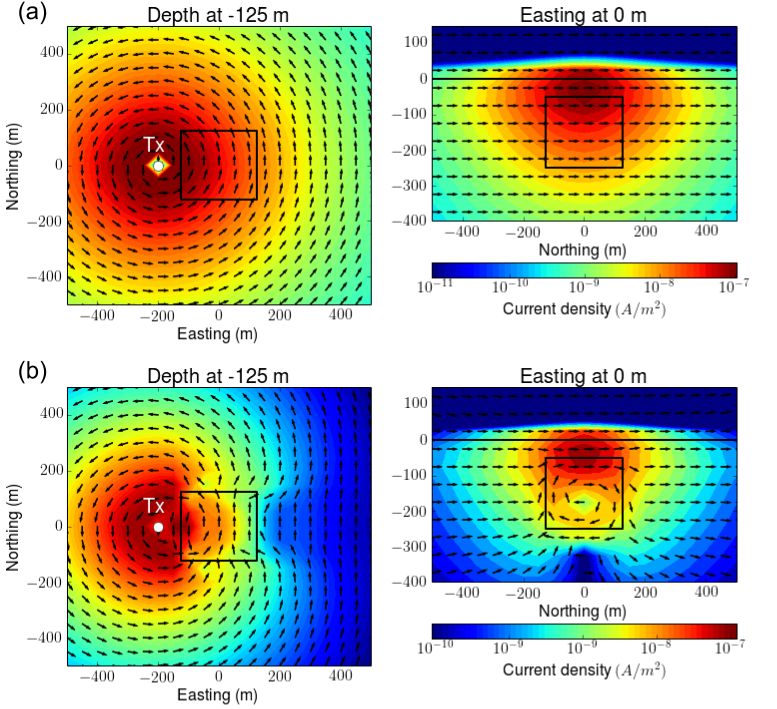
\includegraphics[width=1\textwidth]{figures/ReferenceCurrent.png} }
  \caption{Maps of reference currents: (a) canonical and (b) conductive models. Left and right panel show plan and section views at -125 m-depth and 0 m-easting, respectively. A transmitter is located at (-200 m, 0 m, 30 m). Black arrows and shaded value indicate the direction and amplitude of the current, respectively. Black solid outlines boundary of the surface or the chargeable body.}
  \label{F:ReferenceCurrent}
\end{figure}

\begin{figure}
  \figbox*{}{}{
  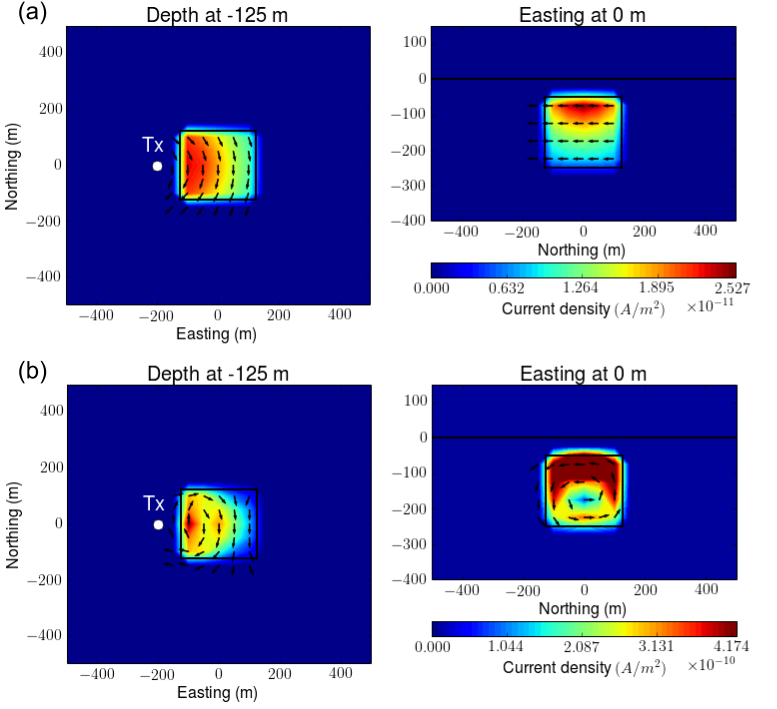
\includegraphics[width=1\textwidth]{figures/Polarizationcurrent_early.png} }
  \caption{Maps of polarization currents: (a) canonical and (b) conductive models at 0.86 ms. Left and right panel show plan and section views at -125 m-depth and 0 m-easting, respectively. A transmitter is located at (-200 m, 0 m, 30 m). Black arrows and shaded value indicate the direction and amplitude of the current, respectively. Black solid outlines boundary of the surface or the chargeable body.}
  \label{F:Polarizationcurrent_early}
\end{figure}

\begin{figure}
  \figbox*{}{}{
  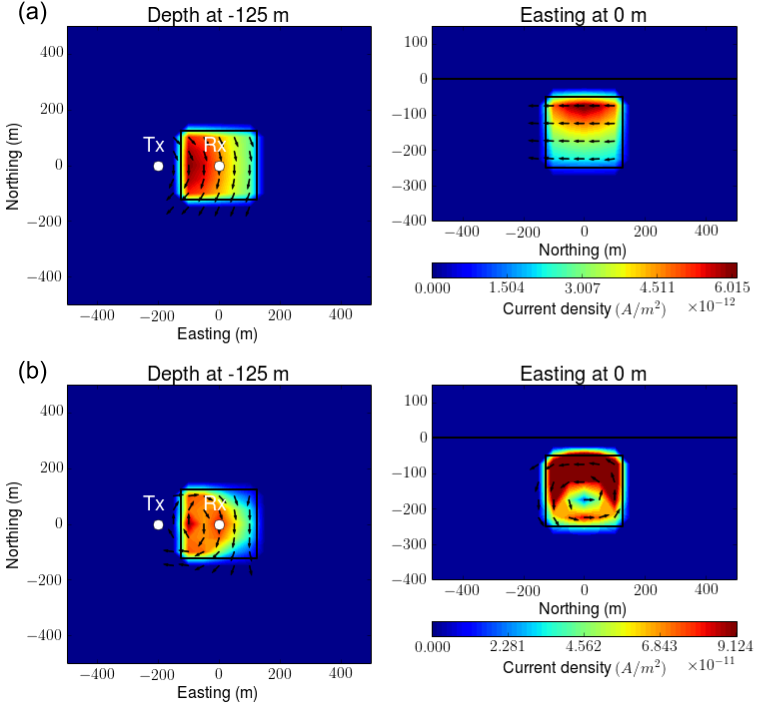
\includegraphics[width=1\textwidth]{figures/Polarizationcurrent_late.png} }
  \caption{Maps of polarization currents: (a) canonical and (b) conductive models at 6.7 ms. Left and right panel show plan and section views at -125 m-depth and 0 m-easting, respectively. A transmitter is located at (-200 m, 0 m, 30 m). Black arrows and shaded value indicate the direction and amplitude of the current, respectively. Black solid outlines boundary of the surface or the chargeable body.}
  \label{F:Polarizationcurrent_late}
\end{figure}
\clearpage

%%% ===========================================================================
%%% SUBSECTION
\subsection{IP currents}
Different from \cite{Smith1988a}, we consider $\siginf \e^{IP}$ term to evaluate the IP current in the linear functional. Relative strength of this term in the IP current to the polarization current is always significant at the outside of the body, because the polarization current is zero. 
An assumption made to evaluate $\e^{IP}$ was ignoring inductive portion in $\e^{IP}$. 
This assumption can be mathematically represented with Helmholz decomposition. 
Using this decomposition, we decompose the IP electric field as $\e^{IP} = - \vec{a}^{IP} -\grad \phi^{IP}$ with $\div \vec{a}^{IP} = 0$. Here $\phi^{IP}$ and $\vec{a}^{IP}$ correspondingly indicate electric scalar and vector potentials; they are galvanic and inductive portions of $\e^{IP}$, respectively. With this decomposition, the IP current can be expressed as $\j^{IP} = \j^{pol}-\siginf \grad \phi^{IP}-\siginf \vec{a}^{IP}$. Relative strength of $-\siginf \vec{a}^{IP}$ compared to two other terms can provide a qualitative measure for the reliability of our assumption. 
Figure ~\ref{F:IPcurrents_helmholtz_early} respectively show plan view maps of $\j^{pol}$, $-\siginf \vec{a}^{IP}$, and $-\siginf \phi^{IP}$ for (a) canonical, (b) conductive, and (c) resistive models at 0.86 ms.
For all three cases the polarization currents have the greatest strength in the body. 
Two other terms related to $\e^{IP}$ exists both in and outside of the body. 
Compared to $-\siginf \grad\phi^{IP}$, $-\siginf \vec{a}^{IP}$ show minor strength for all three cases except for the conductive case. 
For conductive cases both galvanic and inductive portions of the IP current are considerable. 
To examine contributions of each IP current on IP responses, we separately apply Biot-Savart law to each current for the condutive case. 
Figure ~\ref{F:DecompjIPcond} shows IP responses computed from the polarization current (stars), galvanic (rectangles) and inductive portions (circles) of the IP current. Here solid and empty markers show negative and positive signs, respectively. 
The polarization current has major contribution to the IP response, and even IP response due to this current is even greater than true one; they have same sign.
In constrast, galvanic portion of IP responses has opposite sign to them, and its relative strength to the true IP response is getting more significant as time goes later. 
At 6.7 ms, amplitude of IP response due to the polarization current is about 130 percent of the true one, while galvanic portion is 30 percent. 
This result alludes possible collapse of \cite{Smith1988a} assumption as time goes later, while our approach will gets better. 
Inductive portion of IP responses always shows minor contribution compared to galvanic portion except for the time before 0.2 ms, and hence ignoring this inductive portion is reasonable for this case. 

\begin{figure}
  \figbox*{}{}{
  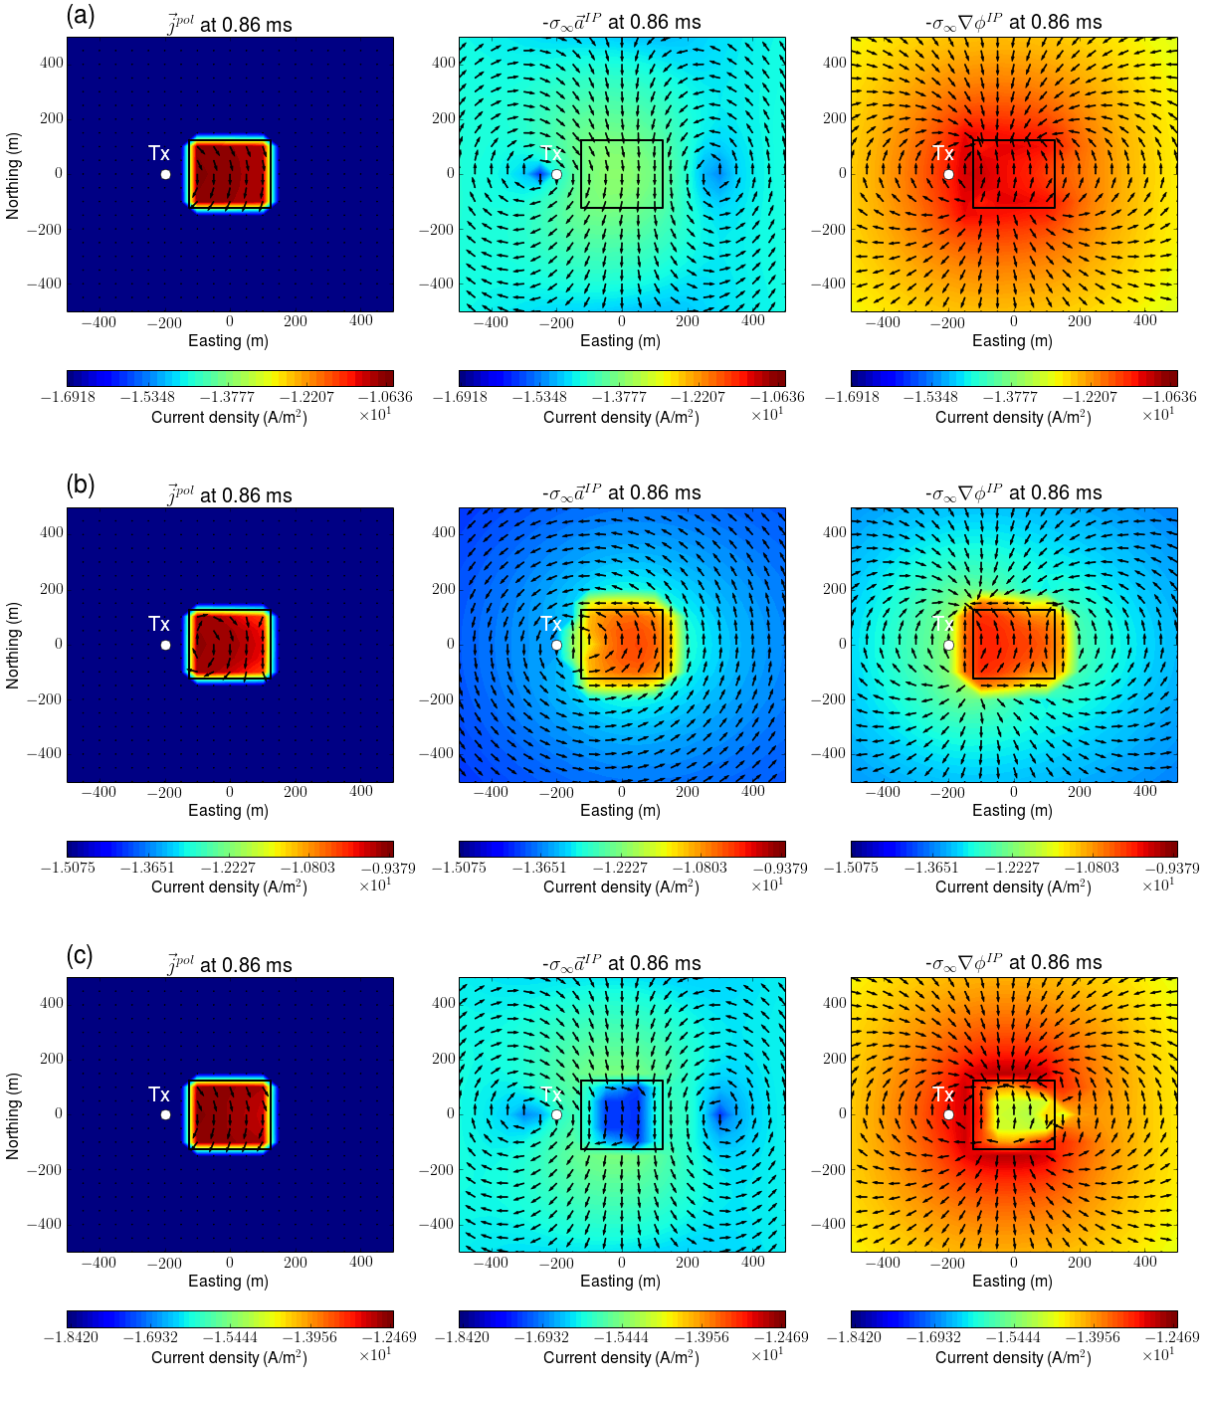
\includegraphics[width=1.\textwidth]{figures/IPcurrents_helmholtz_early.png} }
  \caption{Decomposition of the IP currents as $\j^{pol}$ (left panel), $-\siginf\grad \phi^{IP}$ (middle panel), and $-\siginf\vec{a}^{IP}$ (right panel) at 0.86 ms. Plan view maps of the currents at -125 m-depth are shown. (a) Canonical, (b) Conductive, and (c) Resistive cases. }
  \label{F:IPcurrents_helmholtz_early}
\end{figure}

\begin{figure}
  \figbox*{}{}{
  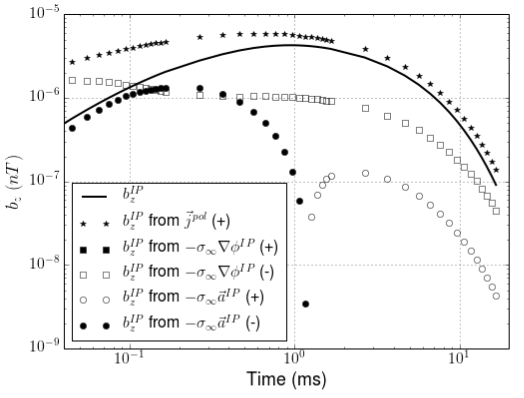
\includegraphics[width=1\textwidth]{figures/DecompjIPcond.png} }
  \caption{Comparisons of contributions of $\j^{pol}$, $-\siginf\grad \phi^{IP}$, and $-\siginf\vec{a}^{IP}$ to the observed IP responses. Solid line indicates true $b_z^{IP}$ responses. Stars, rectangles, and circles correspondingly indicate each IP response genrated by applying Biot-Savart law to $\j^{pol}$, $-\siginf\grad \phi^{IP}$, and $-\siginf\vec{a}^{IP}$. Empty and solid markers represent positive and negative values, respectively. }
  \label{F:DecompjIPcond}
\end{figure}
\clearpage

%%% ===========================================================================
%%% SUBSECTION
\subsection{Validations of linearization}
Our linear functional include two important steps: linearize IP current then apply Biot-Savart law to compute IP responses.
To validate this linear functional, we first compute approximate IP currents using equation (\ref{eq: jip_approx}), and then compare with the true one.
Given that the conductive case is the most complicated situation to expect due to the induced vortex current in the conductor, here we limit our attention only to this case.
Figures ~\ref{F:IPcurrent_PlanandSec_early} show comparison of the true and approximate IP currents for conductive case at 0.86 ms. 
Approximate IP currents show good match with true IP currents in the body about both its direction and amplitude, whereas they show some discrepancy as further away from the body (right panel of Figure ~\ref{F:IPcurrent_PlanandSec_early}).
As time increases to 6.7 ms, approximate current converges to true one as shown in Figure ~\ref{F:IPcurrent_PlanandSec_late}. Similarly, canonical and resistive cases show good matches between the true and approximate IP currents at these times, although we have not shown here. 

Also, we evaluate IP responses by applying Biot-Savart law to approximate IP currents as shown in equation (\ref{eq: BiotbIP_approx}). 
Figure ~\ref{F:True_vs_approx_IPresp} show comparisons of IP responses for canonical (black), conductive (blue), and resistive (red) cases computed by applying discrete Biot-Savart operator to true (solid stars) and approximate (empty circles) IP currents. 
To test the reliability of discrete Biot-Savart operation, we also compute the true IP response by the subtraction of the fundamental response from the observation.
After 0.01 ms, IP responses computed from true IP currents with Biot-savart law almost identical to true IP responses.
Approximate IP response for canonical and resitive cases almost identical to true one after 0.03 ms whereas that for conductive case coverges to true one after 0.8 ms. 
These results consistent with that the canonical and resistive cases have earlier maximum charging time ($\sim$ 0.1 ms) than conductive case ($\sim$ 1 ms).
Overall, developed linear functional for the ATEM data show good performances for all three different conductivity structures in discharging phase. 

Our linear functional reasonably explains $\dip$ data for the resistive case. However, possibility to observe IP response for the resistve case is significantly low considering its small amplitude compared to fundamental response. 

\begin{figure}
  \figbox*{}{}{
  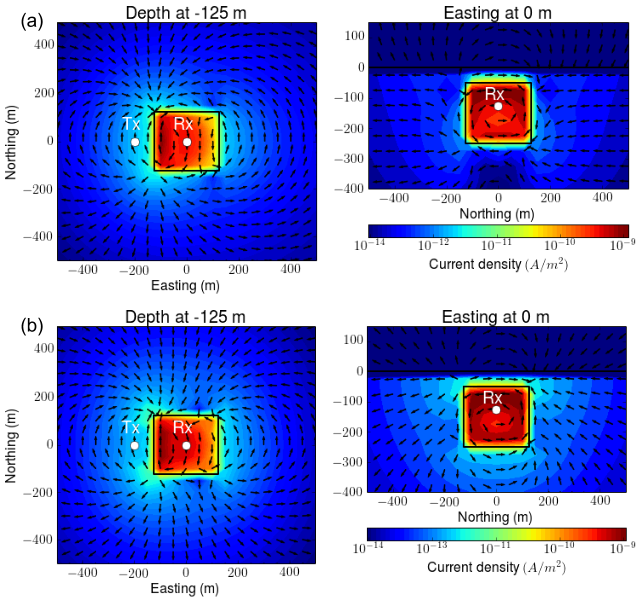
\includegraphics[width=1\textwidth]{figures/IPcurrent_PlanandSec_early.png} }
  \caption{Interpolated maps of (a) true and (b) approximate IP currents at 0.86 ms. Left and right columns show plan and section view maps at -125 m-depth and 0 m-easting, respectively. }
  \label{F:IPcurrent_PlanandSec_early}
\end{figure}

\begin{figure}
  \figbox*{}{}{
  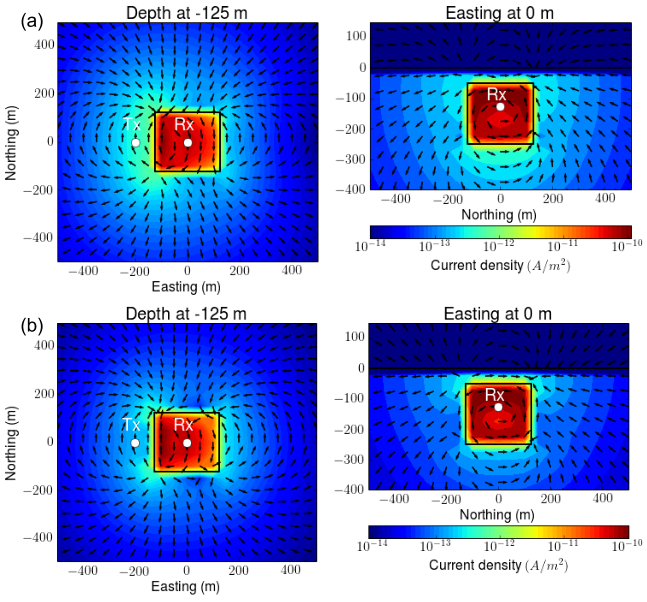
\includegraphics[width=1\textwidth]{figures/IPcurrent_PlanandSec_late.png} }
  \caption{Interpolated maps of (a) true and (b) approximate IP currents at 6.7 ms. Left and right columns show plan and section view maps at -125 m-depth and 0 m-easting, respectively. }
  \label{F:IPcurrent_PlanandSec_late}
\end{figure}

\begin{figure}
  \figbox*{}{}{
  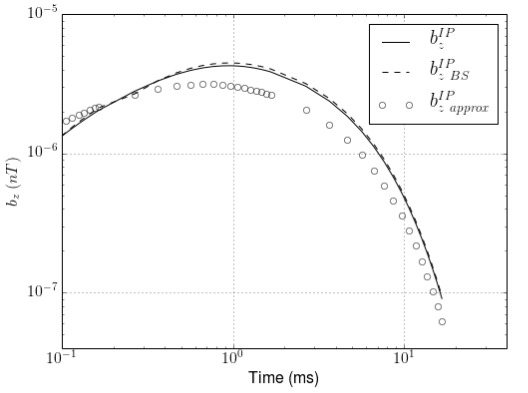
\includegraphics[width=1\textwidth]{figures/True_vs_approx_IPresp.png} }
  \caption{Comparison of true and approximate IP respones ($b_z^{IP}$). Black, blue, and red color respectively indicate canonical, conductive, and resistive cases. Solid lines indicate true $b_z^{IP}$ computed by subtraction process and application of Biot-Savart to true IP current ($b_{z \ BS}^{IP}$). Empty circles presents approximate $b_z^{IP}$. }
  \label{F:True_vs_approx_IPresp}
\end{figure}
\clearpage


%%% ===========================================================================
%%% SUBSECTION
\subsection{Effective pseudo-chargeability for ATEM data}
\label{subsection: Effective pseudo-chargeability for ATEM data}
Using the effective pseudo-chargeability, we altered the problem as shown in equation (\ref{eq: dipeff_kthTx}), which later enables inverse problem recovering not pseudo-chargeability for each transmitter, but an effective pseudo-chargeability. Mathematical formulations to define the effective pseudo-chargeability is described in Section \ref{subsection: Handling multiple transmitters in ATEM surveys}. There we derived the effective pseudo-chargeability by minimizing the squared difference between two quantities shown in equations (\ref{eq: dip_hat}) and (\ref{eq: dip_tilde}). These quantities were not separate $\dip$ datum for each transmitter, but summation for contribution of a single pixel to $\dip$ data for all transmitters. 
Therefore, evaluating this effective pseudo-chargeability, computing IP responses at all transmitter locations, then comparing these to true IP responses are necessary procedure to test feasibility of the effective pseudo-chargeability. 
We only apply this to the conductive model. 

For this test, we first evaluate effective $w^e(t)$ (equation (\ref{eq: we_eff})) then by convoluting $\peta^I(t)$ we compute effective $\peta(t)$. 
This requires calcuating normalized weights shown in equation (\ref{eq: normalized_weights}). 
Figure ~\ref{F:NormalizedWeights} show normalized weights at a single pixel located at (0 m,0 m,-75 m). Reflecting the behaviour of the sensitivity function, the normalized weight is decaying from this pixel. 
With these weights, we compute effective $w^e(t)$ at the same pixel using equation (\ref{eq: we_eff}). 
In Figure ~\ref{F:AveragedWe}, we present $w^e(t)$ (dashed lines) for every transmitter and effective $w^e(t)$ (solid line).
The effective $w^e(t)$ is dominantly affected by the $w^e(t)$ at the center transmitter location (solid circles). Values on early time for this $w^e(t)$ are zero, which are results of projection shown in equation (\ref{eq: we}).
Similarly we evaluate effective $w^e(t)$ for every cell in the domain, and using this we compute effective pseudo-chargeability.
With this we calcuate approximate IP responses using linear functional (equation(\ref{eq: dIP_lineareq})).
Figure ~\ref{F:EquivPeta_True_Approx} show the comparison of true and approximate IP responses on plan view map at 0.86 ms. Relative distribution of true and IP responses at different transmitter locations is compatible whereas the amplitude of $\dip$ is underestimated; the maximum amplitude of the true $\dip$ is $\sim$2 times greater than that of the approximate $\dip$. 
After 0.86 ms, distribution of IP response on map view does not change signficantly and both approximate $\dip$ responses show similar performances.
Same anlayses was applied to canonical and resistive cases and showed similar results, although we have not shown here. 

\begin{figure}
  \figbox*{}{}{
  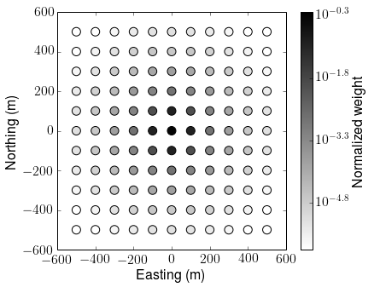
\includegraphics[width=1.\textwidth]{figures/NormalizedWeights.png} }
  \caption{Normalized weights for the conductive case for all trasmitter locations. A single pixel located at (0 m, 0 m, -75 m) is used. }
  \label{F:NormalizedWeights}
\end{figure}

\begin{figure}
  \figbox*{}{}{
  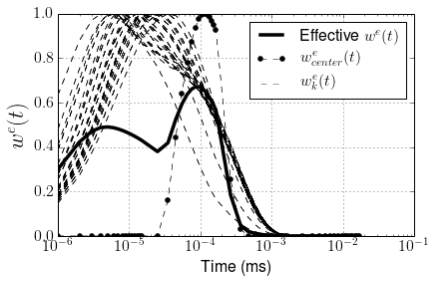
\includegraphics[width=1.\textwidth]{figures/AveragedWe.png} }
  \caption{Effective $w^e(t)$ and $w^e_k(t)$ for all transmitter for the conductive case. A single pixel located at (0 m, 0 m, -75 m) is used.  Solid line and dashed lines correspond to effective $w^e(t)$ and $w^e_k(t)$ for all transmitters ($k=1,\ \ldots,\ nTx$); $w^e_k$ at the center transmitter located at (0 m, 0 m, 30 m) is marked as solid circles. }
  \label{F:AveragedWe}
\end{figure}
\clearpage

\begin{figure}
  \figbox*{}{}{
  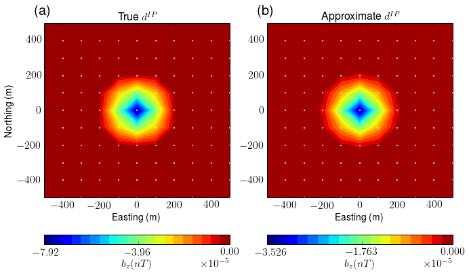
\includegraphics[width=1.\textwidth]{figures/EquivPeta_True_Approx.png} }
  \caption{Comparison of true and approximate $b_z^{IP}$ responses at 0.86 ms on plan view map. }
  \label{F:EquivPeta_True_Approx}
\end{figure}
\clearpage

%%% ===========================================================================
%%% SUBSECTION
\subsection{3D IP inversions}
Using our linearized sensitivty, we now proceed 3D IP inversion, which recovers an effective pseudo-chargeability. For notational convenience, we simply call recovered model from this inversion as pseudo-chargeability for following examples although rigourously, this is effective pseudo-chargeability. 
We limit our attention to the conductive case where the half-space earth includes a body that is conductive and chargeable.
For the computation of the sensitivity we use the true conductivity and then invert data at each  successive time channels and recover 3D pseudo-chargeability at multiple times. 
Our 3D inversion is based upon \cite[]{doug1994,Li2000}, and it requires some choices for inversion parameters. 

For data uncertainties, we used one percent of the maximum amplitude of the observed data (0.1$max(|\mathbf{d}^{obs}|)$). Coefficients for smallness and smoothness are set to $\alpha_s=10^{-5}$ and $\alpha_x=\alpha_y=\alpha_z=1$, respectively. The reference model is zero and we also applied a depth weighting and positivity constraint on the pseudo-chargeablity. 
The need for a depth weighting arises because the sensitivity function $J$ is primarily controlled by a $1/r^3$ decay associated with the Biot-Savart kernels.  Thus an ATEM data set is not unlike commonly acquired  magnetic data where it is well established that a depth weighting is required to image objects at depth. The following example illustrates this. 

We first generate IP responses at a single time using the linear functional by assuming that the pseudo-chargeability is unity inside the body and zero outside, as shown in  Figure \ref{F:Depthweight}(a). 
Figure \ref{F:Depthweight}(b) shows the recovered pseudo-chargeability without depth weighting. 
The recovered anomalous pseudo-chargeability is  at the near surface and the magnitude of the pseudo-chargeability is underestimated ($\sim$0.2). 
By using the depth weighting shown in equation (\ref{eq: weight_mat}),  the IP body is imaged closer to its true depth (Figure \ref{F:Depthweight}(b)). 
Also, the magnitude of the recovered pseudo-chargeability ($\sim$0.6) is closer to the true value than the result without depth weighting. 
Based on this analysis, we use the same depth weighting for our  following examples. 

\begin{figure}
  \figbox*{}{}{
  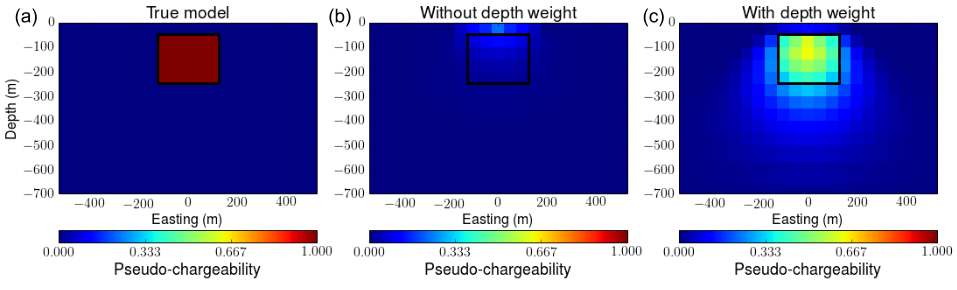
\includegraphics[width=1.\textwidth]{figures/Depthweight.png} }
  \caption{Effect of depth weight in 3D IP inversion. (a) True pseudo-chargeability model on vertical section at 0 m-northing. Recovered pseudo-chargeability models (b) without depth weight and (c) with depth weight.}
  \label{F:Depthweight}
\end{figure}
\clearpage

%%% ===========================================================================
\subsubsection{Incorrect conductivity}
The background conductivity plays a central role in our analysis. It is used in the EM decoupling process and it is also needed to compute the linearized sensitivities for inversion. Since we need to estimate this, usually through the inversion of EM survey data, it will never be correct. Here we explore some effects of an incorrect conductivity but  the consequences are problem dependent.

We return to our conductive block in a halfspace and evaluate the $\dip$ data when the background is the true value ($\sigma_1 = 10^{-3}$ S/m) as well as a factor of two too large (2$\times10^{-3}$ S/m) and a factor of two too small (5$\times10^{-4}$ S/m). The data along a survey line are plotted in Figure \ref{F:Reg_IPresp}.

We invert these three IP responses, and provide sections of the recovered pseudo-chargeability at 0 m-northing. 
Figure \ref{F:Regional_IPInv}(a), (b) and (c) correspondingly show the recovered pseudo-chargeability when the conductivity is: the true value, too high, or too low.  
With the correct conductivity the geometry of the IP body is reasonably recovered. 
When the conductivity is too high, the $\dip$ have a negative bias that results in larger pseudo-chargeabilities and positive-valued artifacts near the IP body (Figure \ref{F:Regional_IPInv}(b)).  
When the conductivity is too small, the IP data have a positive bias and this produces  negative-valued artifacts near the IP body (Figure \ref{F:Regional_IPInv}(c)). However, based on the  definition of the pseudo-chargeability shown in equation (\ref{eq: petaeff_pos}), the sign of the pseudo-chargeability should be positive. By incorporating positivity as a constraint in the inversion we obtain the result in  Figure \ref{F:Regional_IPInv}(d).  This is a much better result and comparison of the observed and predicted data for this case shown in Figure \ref{F:Reg_obspred} clearly shows how this constraint prevents the fitting of positive residual fields. We shall use this positivity  constraint for our following 3D IP inversion examples. 

The background conductivity is also needed when computing the sensitivity function, since we need the reference electric field, which is dependent on conductivity. 
An incorrect conductivity will affect the sensitivity function as well. 
In order to test this, we compute the sensitivity  matrix using a half-space conductivity model ($\siginf = \sigma_1$). 
Figure \ref{F:True_vs_approx_sensitivity} compares the recovered pseudo-chargeability from the 3D IP inversion of the IP datum at 1.0 ms with the true and incorrect sensitivity function using half-space conductivity. 
There is not a large difference between the two inversions  which suggests that an approximate conductivity may still provide sensitivities that are adequate for inversion. This parallels results from EIP where even an approximate conductivity can still yield good results when inverting the data. Thus there is some robustness in our sensitivity function with respect to an  incorrect conductivity and even if we  not have an accurate 3D conductivity model we can still apply our 3D IP inversion using half-space conductivity so long as the ATEM data includes distinctive IP response such as negative transients.

% On the other hand, in above examples we inverted true $\dip$ data, and for each inversion we recovered a subset of effective pseudo-chargeability.
% Although the reliability of altering an inverse problem using an effective pseudo-chargeability was demonstrated in Section \ref{subsection: Effective pseudo-chargeability for ATEM data}, investigation of a recovered pseudo-chargeability from the inversion is necessary.
% The recovered pseudo-chargeability shown in Figure ~\ref{F:Regional_IPInv}a from true $\dip$ data show proper geometry of the true chargeable body, which strengthen the feasiblity of our method. 

\begin{figure}
  \figbox*{}{}{
  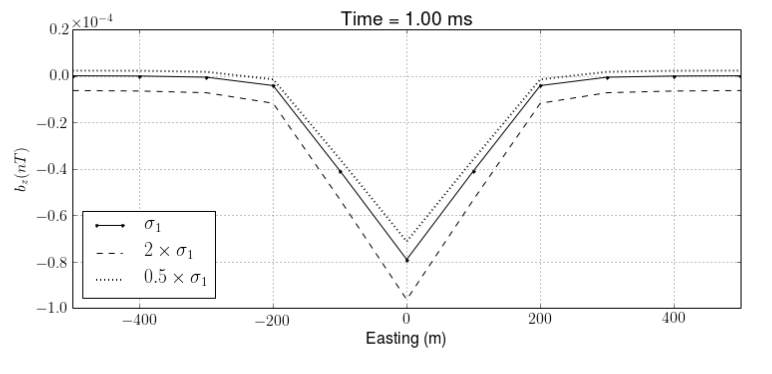
\includegraphics[width=1.\textwidth]{figures/Reg_IPresp.png} }
  \caption{IP responses on a profile line at 0 m-northing.  IP responses are computed from perturbed $\siginf$ models. Half-space conductivity ($\sigma_1$) is perturbed two times higher or less resulting in overestimated (dotted line) and underestimated (dashed line) IP respones. Solid line shows the true IP response. }
  \label{F:Reg_IPresp}
\end{figure}

\begin{figure}
  \figbox*{}{}{
  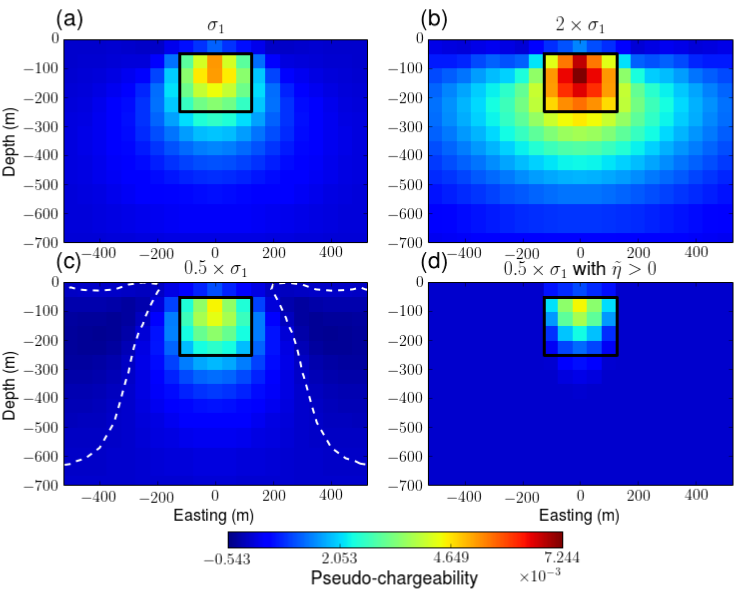
\includegraphics[width=1.\textwidth]{figures/Regional_IPInv.png} }
  \caption{Recovered pseudo-chargeability sections from 3D IP inversions at 0 m-northing. (a) $\dip$ with true $\sigma_1$. (b) $\dip$ with 2$\times \sigma_1$. (c) $\dip$ with 0.5$\times \sigma_1$. (d) $\dip$ with 0.5$\times \sigma_1$ and the positivity constraint on the pseudo-chargeability. White dashed lines contour zero-crossing lines.}
  \label{F:Regional_IPInv}
\end{figure}

\begin{figure}
  \figbox*{}{}{
  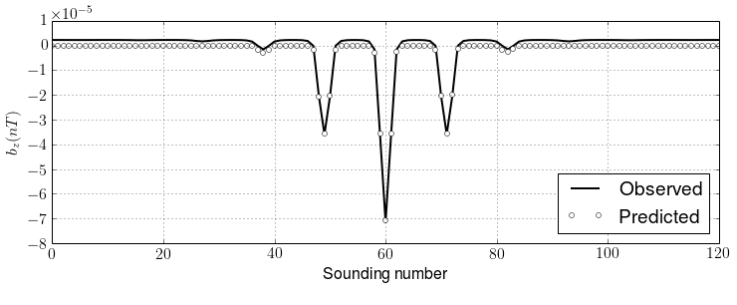
\includegraphics[width=1.\textwidth]{figures/Reg_obspred.png} }
  \caption{Comparison of the observed (solid line) and predicted (empty circles) data. $\dip$ response was generated with underestimated half-space conductivity (0.5$\times \sigma_1$). The positivity constraint was used the 3D IP inversion.}
  \label{F:Reg_obspred}
\end{figure}

\begin{figure}
  \figbox*{}{}{
  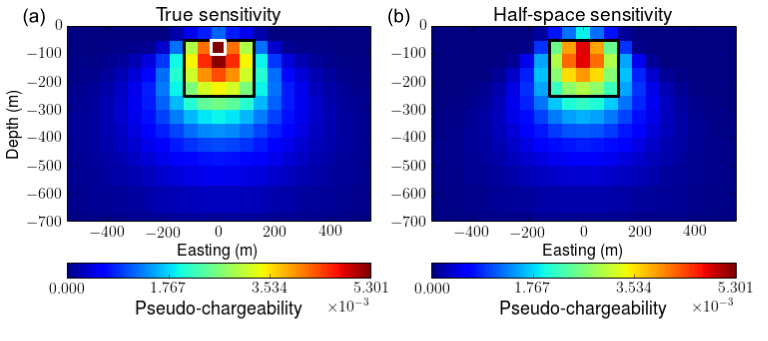
\includegraphics[width=1.\textwidth]{figures/True_vs_approx_sensitivity.png} }
  \caption{Recovered pseudo-chargeabilty sections from the 3D IP inversions at 0 m-northing.  (a) True and (b) incorrect $\siginf$ is used to compute sensitivity function. For the incorrect sensitivity we used half-space conductivity ($\sigma_1$).}
  \label{F:True_vs_approx_sensitivity}
\end{figure}
\clearpage

%%% ===========================================================================
\subsubsection{Extracting intrinsic IP parameters}
By applying our inversion to each time channel of $\dip$ data separately, we can recover 3D distributions of pseudo-chargeability at multiple times. 
Pseudo-chargeability at each time carried different information about the state of polarization and we can use these to recover information about intrinsic IP parameters. 
Diverse time-dependent conductivity models such Cole-Cole model and stretched-exponential can be used for this interpretation.
We use the Cole-Cole model with $c$=1. 
We parametrize pseudo-chargeability at a single pixel in terms of chargeability and time constant as described in Section \ref{section: extract_intrinsicIP}, and solve a small inverse problem. This parallels \cite[]{Yuval1997,Hordt2006}.

As an example, use the conductive and chargeable block presented in the previous section and we invert 14 time channels of data ranging from 1-10 ms.  The true $\siginf$ model is used  for both evaluation of IP datum and sensitivity function. The recovered pseudo-chargeability from one of the 14 inversions is shown in Figure \ref{F:True_vs_approx_sensitivity}a. In that pseudo-chargeability model, we choose cells having greater pseudo-chargeability value than 0.001, and estimate the time constant ($\tau$) and chargeability ($\eta$) of each cell separately. 
A forward kernel for this inversion is shown in equation (\ref{eq: pseudochargeability_petaI}), which requires effective $w^e(t)$. 
The effective $w^e(t)$ for this pixel are shown in Figure \ref{F:AveragedWe}, and this is used to evaluate the forward kernel for the inversion.
Figure ~\ref{F:EtaTauSection}a and b correspondingly show the estimated time constant and chareability on section view maps.
Estimated time constant values show reasonable values in overall region compared to the true value: 0.005. 
Near upper boundary of the chargeable body, estimated chareability is around 0.1, which is 2 times less than the true value: 0.2, and away from this region estimated values are considerably underestimated. 
This result is possibly related to greater sensitivity of IP response for the ATEM data on near surface chargeable medium. å
In Figure \ref{F:IntrinsicIP}, we also proivde time decay of the observed and predicted data at a single pixel marked as black empty rectangles in Figure ~\ref{F:EtaTauSection}.
The estimated time constant ($\tau_{est}$) and chargeability ($\eta_{est}$) for this pixel are 0.0044 and 0.11, respectively. 
These results imply more stability on recovering time constant than chargeability with our approach. Although the same experiments for canonical and resistive cases have been treated, we have not shown here for the brevity of the article.
Similar to conductive case, we recovered reasonable time constant, whereas the recovered chargeability is underestimated for two other cases. 

We used a simple interpretation method to extract Cole-Cole parameters from multiple times of recovered pseudo-chargeability, which are products of our IP inversion, to glimpse a possibility on this problem. 
However, more sophisticated methodology and systematic analayses on extracting this intrinsic IP information from $\dip$ data are necessary as a future study. 

\begin{figure}
  \figbox*{}{}{
  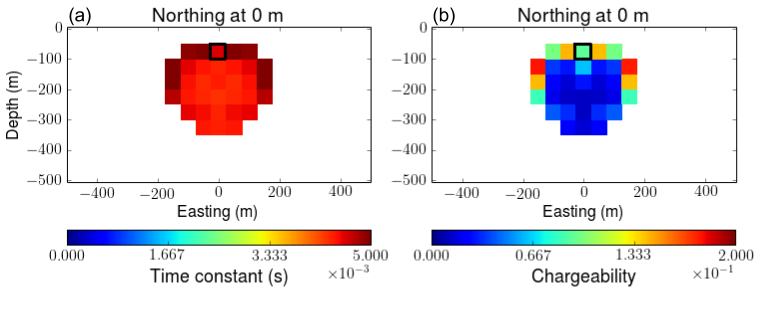
\includegraphics[width=1.\textwidth]{figures/EtaTauSection.png} }
  \caption{Section views of recovered (a) time constant and (b) chargeability. Any region where the peudo-chargeabiliy shown in Figure ~\ref{F:True_vs_approx_sensitivity}a is smaller that 0.001 is ignored this analysis, and blanked.}
  \label{F:EtaTauSection}
\end{figure}

\begin{figure}
  \figbox*{}{}{
  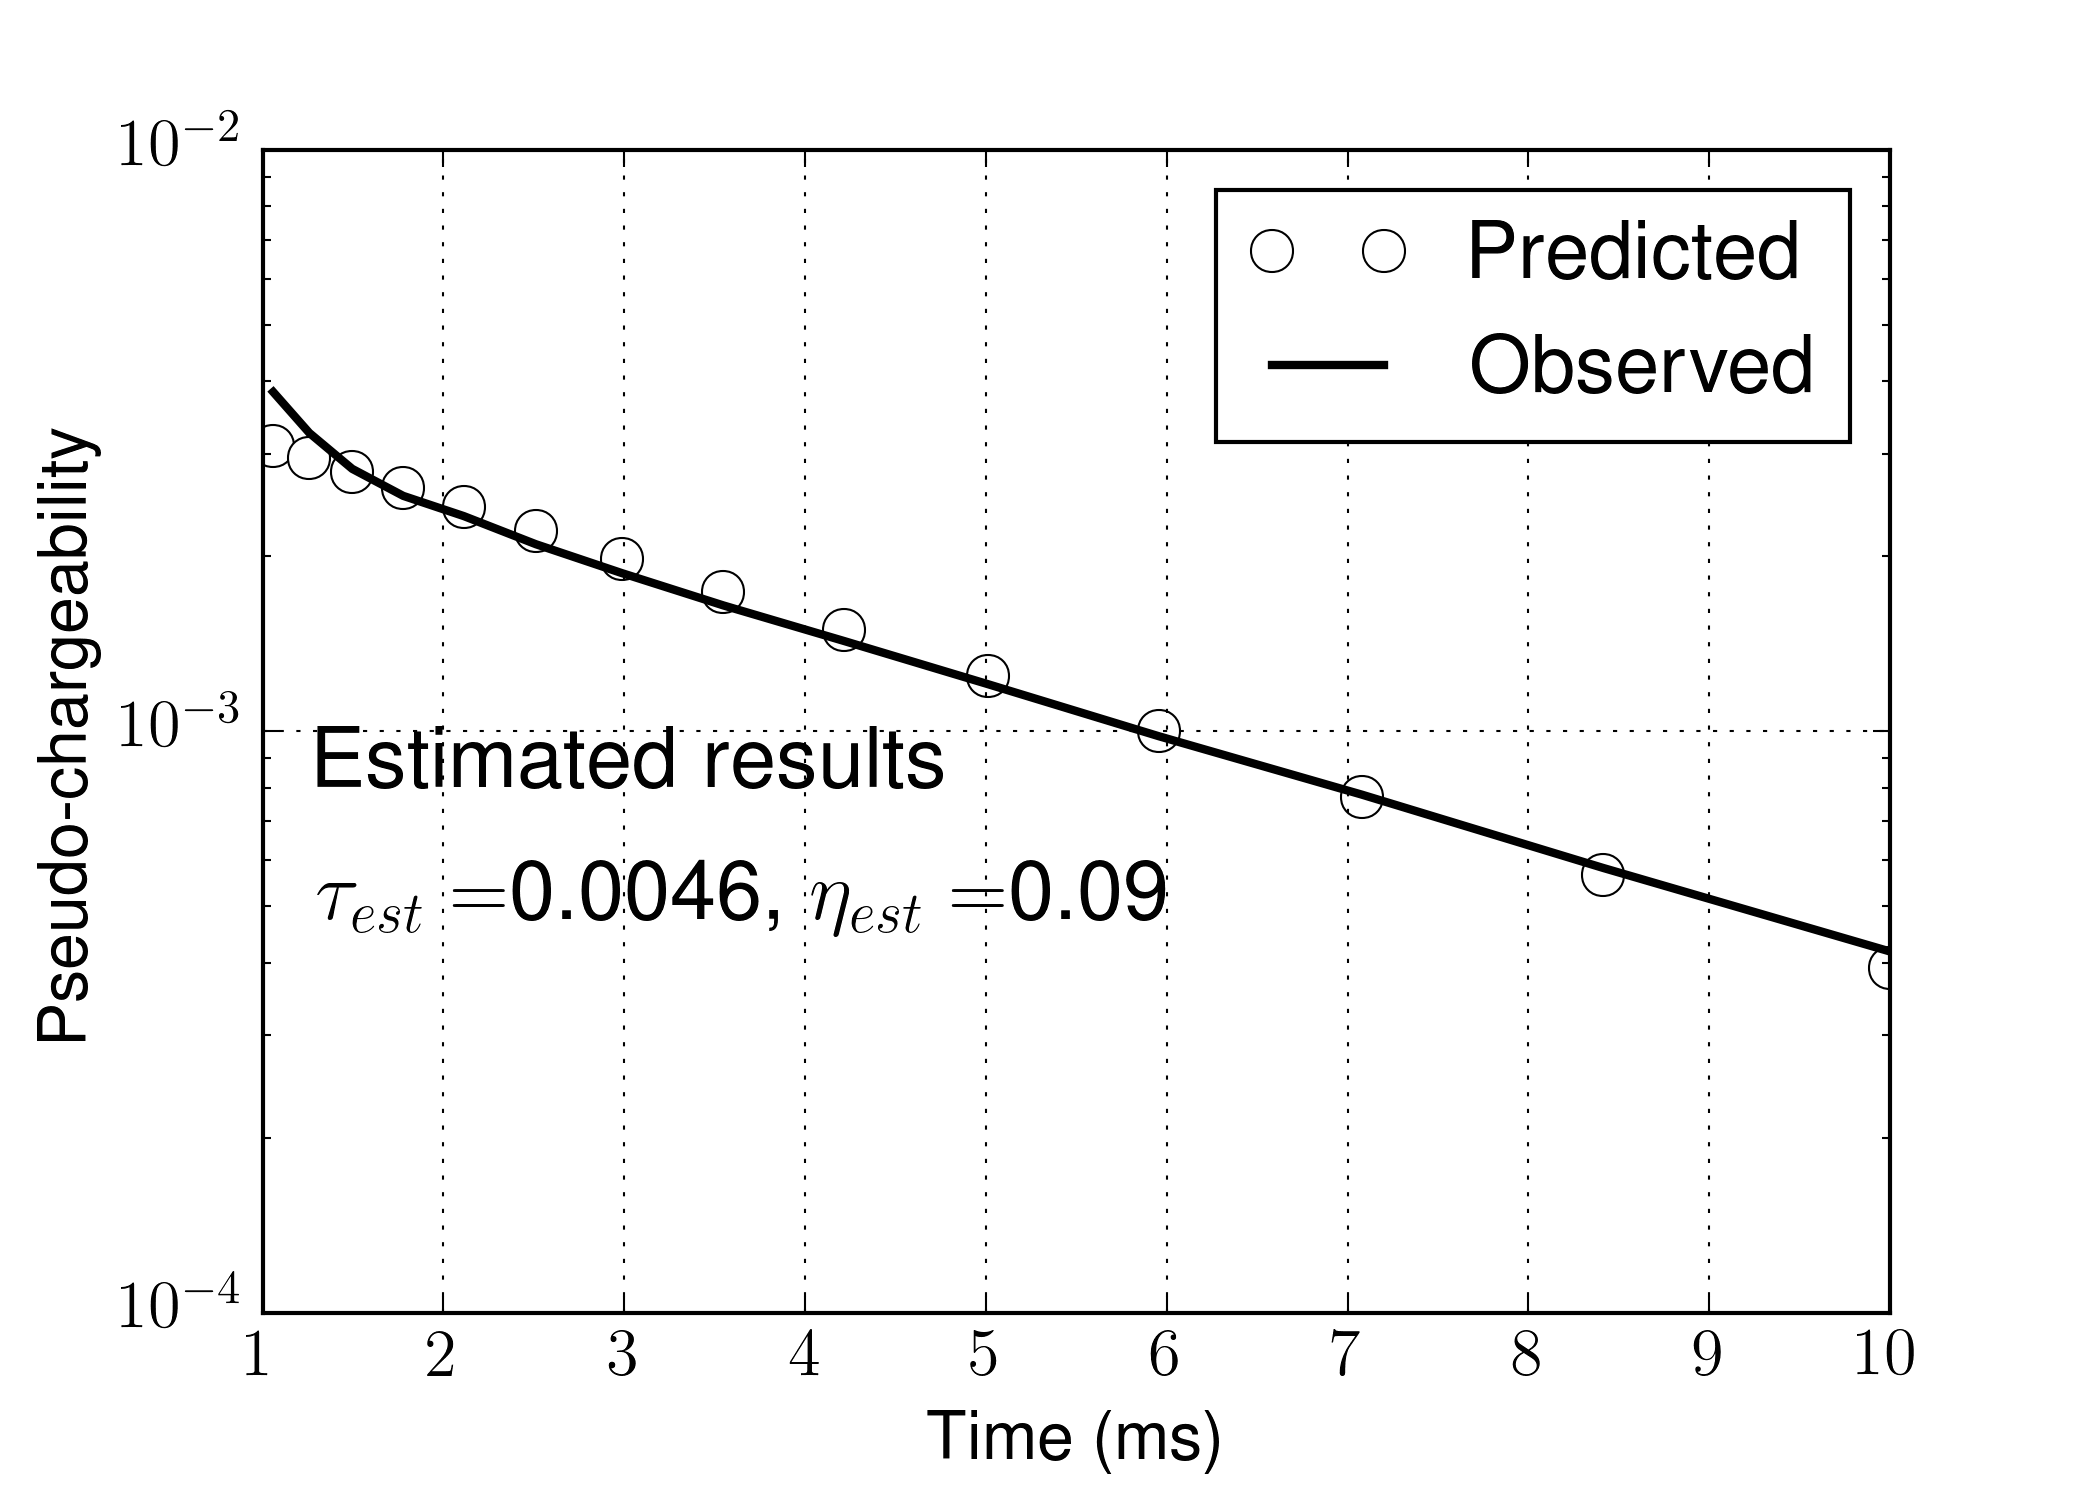
\includegraphics[width=1.\textwidth]{figures/IntrinsicIP.png} }
  \caption{Comparisons of the observed and predicted pseudo-chargeability at a single pixel in a chargeable body. 
  Empty and solid circles indicate predicted pseudo-chargeabilities using two different $w^e_{avg}(t)$ for the choices of normalized weights: a single cell and all cells in a chargeable block, respectively. Estimated time constant and chargeability for each inversion are expressed as $\tau_{est}$ and $\eta_{est}$, respectively.}
  \label{F:IntrinsicIP}
\end{figure}
\clearpage

%% =============================================================================
%% Section. Conclusions
%% =============================================================================
\section{Conclusions}
In this paper, we have introduced an IP inversion procedure for the TEM data, especially for the inductive source. 
This includes three main steps: 1) subtraction of the fundamental response from the observation, 2) linearization of the IP response as a function of the pseudo-chargeability, and 3) restoration of 3D pseudo-chargeability at multiple times, and further interpretation of the pseudo-chargeability to extract intrinsic IP parameters like Cole-Cole model. We used ATEM survey to test our IP inversion procedure.

Assuming that we can recover reasonable 3D conductivity by inverting TEM data with exception of the IP-contaminated data, evaluation of the first step allows us to identify IP responses embedded in the observation. 
By taking analogy from the EIP case, we effectively linearize ISIP response in time domain as a function of the pseudo-chargeability. 
This pseudo-chargeability is defined as a fraction of the polarization current and the reference current, which may provide us the strength of the IP effect. 
Different from the EIP case, the polarization charge buildup does not reach to the steady-state for the ISIP case due to the absence of steady-state electric field for inductive source. 
This fundamental difference is carefully incorporated to the linearization with a proper choice of the reference electric field. 
Numerical tests on the approximate IP current and responses demonstrated the capability of the linearized kernel for various conductivity structures: canonical, conductive, and resistive cases. 
Our linearization is effective at certain late time when the IP effect is considerable to the EM effect, which may occur in the discharging phase. 

In order to formulate 3D IP inversion, we derived an effective pseudo-chargeability, which represents pseudo-chargeability of every transmitter, and tested with numerical simulation. 
Based on this, we inverted IP responses at multiple times, separately, and recovered pseudo-chargeability at those times.
Due to the possible lack of intrinsic depth resolution in our kernel for the ATEM survey, the depth weighting is used in the inversion.  
Our 3D IP inversion recovered reasonable geometric shape and location of the chargeable body. 
Because we may not recover true conductivity in practice, we tested possible effects of incorrect conductivity. 
Two important places where we use conductivity are EM decoupling and sensitivity function. 
By designing two situations where we have postive or negative residual field in the IP response, we investigated the effect of incorrect conductivity in the IP response and the 3D IP inversion. 
For the positive residual field, we showed that positivity constraint can be effectively used to prevent fitting those residual field. 
In addition, even with a poor sensitivity function computed using half-space conductivity model, we recovered important information of the chargeable body such as geometric shape and location . 
Finally, by interpreting recovered pseudo-chargeability at the center pixel of the IP body in time, we extracted Cole-Cole parameters: $\tau$ and $\eta$ by assuming $c=1$. 
Estimated $\tau$ was close to true one whereas $\eta$ was underestimated.
This suggests a potential to extract intrinsic IP parameters from the recovered pseudo-chargeability. 

Our IP inversion procedure provides a framework that one can recover 3D distribution of the pseudo-chargeability, and possibly extraction of intrinsic IP parameters with post-processings of the pseudo-chargeability. 
Because our inversion procedure requires 3D distribution of $\siginf$, which may not be trivial in some cases, this should be carefully investigated in the future for practical application of our inversion methodology. 
In addition, our numerical examples was only treated the ATEM survey, even though application to different types of inductive source TEM survey such as Large-loop TEM may have different aspects that we need to consider. 
However, still important items including EM decoupling, linearization and 3D IP inversion, which have been come up with and carefully tested in this study, will be fundamental backgrounds of following future studies about the ISIP in time domain. 

% =======================================================================
% SECTION (Appendix)
% =======================================================================
\appendix
%%% ===========================================================================
%%% SUBSECTION
\section{Discretization of steady-state Maxwell's equations}
\label{section:maxwell_discrete}
As shwon equation (\ref{eq: phiIPapprox_general}), computation of our linearized kernel requires solving steady-state Maxwell's equations. 
We discretize this system using mimetic finite volume (FV) method with weak formulation (\cite{Eldadbook}). 
For the discretization, we assume that the electric field $\e$ is discretized by grid function $\de$ on cell edges and magnetic flux density $\b$ is discretized by grid fuction $\db$ on cell faces. 
Electrical potential $\phi$ is discretized by grid fucntion  $\phi$ on cell nodes. For clear representation of the derivation, recall Maxwell's equations in steady state as
\begin{align}
  \j = \siginf\e = -\siginf\grad \phi, \\
  -\div \j = \div \j_s, \\
  \j\big|_{\partial \Omega}\cdot\hat{n} = 0,
  \label{eq:DCBCneumann}
\end{align}
where $\partial \Omega$ indicates boundary surface of the system and $\hat{n}$ is the normal vector of the boundary surface. Weak form of those equations can be written as
\begin{align}
  (\j, \vec{w}) + (\siginf \grad \phi, \vec{w}) = 0, \\
  -(\j, \grad \psi) = (\j_s, \grad \psi).
\end{align}
The inner products $(\j, \vec{w})$, $(\siginf \grad \phi, \vec{w})$,  $(\j, \grad \psi)$ and $(\j_s, \grad \psi)$ are edge based products. Here we define the inner product as
\begin{linenomath*}
\begin{equation}
  (\vec{a}, \vec{b}) = \int_{\Omega} \vec{a}\cdot\vec{b} dv,
\end{equation}
\end{linenomath*}
where $\Omega$ is the volume of the system. By discretizing $\grad$ operator and the inner product in space, we obtain
\begin{linenomath*}
\begin{equation}
  \Me\dj + \MeSigInf\dgrad\boldsymbol{\phi} = 0,
  \label{eq:DCdisceq1}
\end{equation}
\end{linenomath*}
\begin{linenomath*}
\begin{equation}
  -\dgrad^T \Me\dj = \dgrad^T \Me\dj_s,
  \label{eq:DCdisceq2}
\end{equation}
\end{linenomath*}
where $\mathbf{M}^e_i$ is the mass matrices, which discretize the edge based inner product (\cite{Eldadbook}). This inner products are defined  as
\begin{align}
  \mathbf{M}^e_i = \diag(\Ace^T\diag(\vol)\mathbf{i}).
\end{align}
Here, $\mathbf{i}$ indicates a grid function on cell center like $\siginf$, and $\vol$ is the grid function for the cell volume. The averaging matrix $\Ace$ averages discrete function defined on the edges to the cell center. The mass matrix $\Me$ without subscript $i$ indicates that $\mathbf{i}$ is equal to the identity column vector of which all elements are one. By substituting equation (\ref{eq:DCdisceq1}) to (\ref{eq:DCdisceq2}), we have
\begin{linenomath*}
\begin{equation}
  \A_{\siginf}\boldsymbol{\phi} = \mathbf{rhs}^{DC},
  \label{eq:DCdiscLin}
\end{equation}
\end{linenomath*}
where $\A_{\siginf} = \dgrad^T \MeSigInf\dgrad$ and $\mathbf{rhs}^{DC} = \dgrad^T \Me\dj_s$. 

%% ===========================================================================
%% SUBSECTION
\section{Discretization of the linearized kernel}
\label{section:linearkernel_discrete}
To obtain linear form of equation shown in equation (\ref{eq: dIP_lineareq}),
we first discretize Biot-Savart law shown in equations (\ref{eq: BiotbIP_approx}) and (\ref{eq: BiotbIPdt_approx}). In our discretization $\j^{IP}$ and  $\peta$ are defined on the cell center, and those for each time channel are constant in a cell volume, whereas $\eref$ is defined on the cell edges. 
We define the number of cells and edges in 3D space as nC and nE, respectively. Discretized IP current density, $\dj^{IP}_{cc} \in \mathbb{R}^{3nC}_{1}$, and defined on the cell center, since $\j^{IP}$ has three components, we first discretize integration operator including cross product ($\int_{v}\frac{ \times \hat{r}}{r^2}dv$) as
\begin{linenomath*}
\begin{equation}
  \mathbf{G}_{Biot} =
  \begin{bmatrix}
       \mathbf{e}^T &  \mathbf{0}   & \mathbf{0}  \\
       \mathbf{0}   &  \mathbf{e}^T & \mathbf{0}  \\
       \mathbf{0}   &  \mathbf{0}   & \mathbf{e}^T
    \end{bmatrix}
  \begin{bmatrix}
       \mathbf{0}     &   \mathbf{S}_z   & -\mathbf{S}_y  \\
      -\mathbf{S}_z   &   \mathbf{0}     &  \mathbf{S}_x  \\
       \mathbf{S}_y   &  -\mathbf{S}_x   &  \mathbf{0}
    \end{bmatrix},
\end{equation}
\end{linenomath*}
where
\begin{linenomath*}
\begin{equation*}
  \mathbf{S}_l =\diag(\mathbf{v}\oplus \mathbf{r}_l \oplus \frac{1}{\mathbf{r}^2}), \ l = x, \ y, \ z
\end{equation*}
\end{linenomath*}
and the electric field, $\mathbf{e} \in \mathbb{R}^{nE}_1$ is a column vector, $\diag(\cdot)$ is the diagonal matrix and $\oplus$ is the Hadamard product. 
Then we discretize $\j^{IP}$ shown in equation (\ref{eq: jip_approx}) as
\begin{linenomath*}
\begin{equation}
  \dj^{IP}_{cc}(t) = \mathbf{S}\diag(\de^{F}_{max})\Ace^T\diag(\vol)\diag(\siginf)\peta(t),
\end{equation}
\end{linenomath*}
where
\begin{linenomath*}
\begin{equation}
  \mathbf{S} = \mathbf{A}^{e}_{ccv}\Me^{-1}[\MeSigInf \mathbf{G} \A_{\siginf}^{-1}\mathbf{G}^T  - \mathbf{I}] \diag(\de^{F}_{max})\Ace^T\diag(\vol)\diag(\siginf).
\end{equation}
\end{linenomath*}
and $\mathbf{A}^{e}_{ccv}$ is discrete averaging matrix from edge to cell center with consideration of three component vector: $\in \mathbb{R}^{3nC}_{nE}$. 
Thus, we can have linear equation for $k^{th}$ time channel as
\begin{linenomath*}
\begin{equation*}
  \db^{IP}_i = \Gbiot \mathbf{S} \peta_i,
\end{equation*}
\end{linenomath*}
where subscript $i$ indcates $i^{th}$ time channel. Finally, by letting
\begin{linenomath*}
\begin{equation}
  \mathbf{J} = -\Gbiot\mathbf{S},
  \label{eq: Sense}
\end{equation}
\end{linenomath*}
we have
\begin{linenomath*}
\begin{equation}
  \db^{IP}_i = \mathbf{J}\peta_i,
  \label{eq: bIP_linear}
\end{equation}
\end{linenomath*}
where $\mathbf{J}$ is the Jacobian matrix of the linear equation, and since $\mathbf{J}$ is static, we also obtain
\begin{linenomath*}
\begin{equation}
  -\frac{\partial\db^{IP}}{\partial t}\Big|_i = \mathbf{J}(-\frac{\partial \peta}{\partial t}\Big|_i).
  \label{eq: dbIPdt_linear}
\end{equation}
\end{linenomath*}

\bibliographystyle{gji}
\bibliography{reference}

\end{document}


%%% Dummy

% \subsection{Discrete Helmholtz decomposition}
% \label{section:helmholtz}
% In continuous space, we can decompse arbitrary vector field as 
% \begin{linenomath*}
% \begin{equation}
%   \e = -\grad\phi -\vec{a},
% \end{equation}
% \end{linenomath*}
% where $\div \vec{a} = 0$. 
% Decomposition of discrete electric field, $\de$, can be expressed as
% \begin{linenomath*}
% \begin{equation}
%   \Me\de = -\Me\dgrad \boldsymbol{\phi} -\Me\mathbf{a},
% \end{equation}
% \end{linenomath*}
% where $\boldsymbol{\phi}$ and $\mathbf{a}$ are discrete scalar and vector potentials, respectively. 
% By taking discrete divergece ($-\dgrad^T$), we obtain
% \begin{linenomath*}
% \begin{equation}
%   -\dgrad^T\Me\dgrad\boldsymbol{\phi} = \dgrad^T\Me\mathbf{a} + \dgrad^T\Me\de
% \end{equation}
% \end{linenomath*}
% Since the vector potential $\vec{a}$ is divergece free, the first term in the right-hand side is zero. Thus, we obtain
% \begin{linenomath*}
% \begin{equation}
%   \dgrad^T\Me\dgrad\boldsymbol{\phi} = -\dgrad^T\Me\de. 
% \end{equation}
% \end{linenomath*}
% By solving this linear system we can first compute $\boldsymbol{\phi}$, then by subtracting this from $\de$, we can also obtain the vector potental, $\mathbf{a}$. 
% %% Appendix
% 1. Discretization of the linearized kernel
% 2. Numerical evaluation of the Helmholtz decomposition



